%\documentclass[]{beamer}
\documentclass[aspectratio=169,tikz]{beamer}
%\pdfpkresolution=3600
\usepackage[utf8]{inputenc} % use UTF-8
\usepackage[T2A,OT1]{fontenc} % rus fonts
\usepackage[russian]{babel}

\usepackage{xspace}
\usepackage{lipsum}
\usepackage{standalone}
\usepackage{setspace}
\usepackage{tkz-euclide}
\usepackage{subfigure}
\usepackage{listings} % for code listings

\usetikzlibrary{shapes,backgrounds}
\usepackage{pgf-umlcd}

\tikzstyle{startstop} = [rectangle, rounded corners, minimum width=3cm, minimum height=1cm,text centered, draw=black, fill=red!30]

\tikzstyle{io} = [trapezium, trapezium left angle=70, trapezium right angle=110, minimum width=3cm, minimum height=1cm, text centered, draw=black, fill=blue!30]

\tikzstyle{process} = [rectangle, minimum width=3cm, minimum height=1cm, text centered, draw=black, fill=orange!30]

\tikzstyle{decision} = [diamond, minimum width=3cm, minimum height=1cm, text centered, draw=black, fill=green!30]

\tikzstyle{arrow} = [thick,->,>=stealth]


\usepackage{tkz-euclide}
\usetikzlibrary{shapes,backgrounds}


\tikzset{weird fill/.style={append after command={
			\pgfextra
			\draw[sharp corners, fill=#1,fill opacity=0.3, draw=none]% 
			(\tikzlastnode)% 
			[rounded corners=8pt] -| (\tikzlastnode.west)
			[rounded corners=8pt] |- (\tikzlastnode.north)% 
			[rounded corners=8pt] -| (\tikzlastnode.east)% 
			[rounded corners=8pt] |- (\tikzlastnode.south);
			\endpgfextra}}}

\newcommand\pack[6][]{%
	\path[#1] (#4,#5) -- (#4-#2 , #5)
	-- (#4-#2 ,#5+#3) -- (#4-#2 ,#5+#3 + 0.7)
	-- (#4-#2 + #6 * #2 ,#5+#3 + 0.7) -- (#4-#2 + #6 * #2+0.0 ,#5+ #3)
	-- (#4, #5+#3)
	--cycle;
	\path[#1] (#4-#2 , #5+ #3) -- (#4-#2 + 0.8* #2+0.5 ,#5+ #3);
}

\def\package[#1](#2:#3:#4:#5:#6){%
	% Synopsis                 2  3 4 5 6
	% \package[draw options](text:w:h:x:y)
	%	\pack[draw=black, rounded corners=8pt, thick, fill=white]{#3}{#4}{#5}{#6};
	%	\pack[draw=black, rounded corners=8pt, thick, fill opacity=0.2, #1]{#3}{#4}{#5}{#6};
	%	\node [anchor=west, draw=black, thick] at (#5-#3,  #6+#4+0.35) {\texttt{#2}};	
	
	%	\node [anchor=west] at (#5-#3,  #6+#4+0.35) {\texttt{#2}};
	\draw node[minimum height=5mm,anchor=south west,minimum width=15mm,
	append after command={[rounded corners=8pt](b.west)|-(b.north)},
	append after command={[rounded corners=8pt](b.north)-|(b.east)},
	append after command={[rounded corners=0pt](b.east)|-(b.south)},
	append after command={[rounded corners=0pt](b.south)-|(b.west)}, weird fill=#1]
	(b) at (#5,  #6+#4) {\texttt{#2}};
	
	\draw node[minimum height=5mm,anchor=south west,minimum width=15mm,
	append after command={[rounded corners=8pt](b.west)|-(b.north)},
	append after command={[rounded corners=8pt](b.north)-|(b.east)},
	append after command={[rounded corners=0pt](b.east)|-(b.south)},
	append after command={[rounded corners=0pt](b.south)-|(b.west)}]
	(c) at (#5,  #6+#4) {\texttt{#2}};
	
	
	\path[draw,black,fill=#1,fill opacity=0.3,rounded corners=8pt] (#5, #6 + #4) -- (#5,#6) -- (#5+#3, #6) -- (#5+#3, #6 + #4) -- (#5, #6 + #4);
}



\newcolumntype{Z}{>{\centering\let\newline\\\arraybackslash\hspace{0pt}}X} 
\newcolumntype{M}{>{\raggedright\let\newline\\\arraybackslash\hspace{0pt}}X}
\newcolumntype{L}[1]{>{\raggedright\let\newline\\\arraybackslash\hspace{0pt}}m{#1}}
\newcolumntype{C}[1]{>{\centering\let\newline\\\arraybackslash\hspace{0pt}}m{#1}}

\newcommand{\kmeans}{\mbox{$ k $-means}\xspace}
\newcommand{\Ward}{Ward\xspace}
\newcommand{\AWard}{\mbox{A-Ward}\xspace}
\newcommand{\Wardp}{\mbox{Ward$ _p $}\xspace}
\newcommand{\AWardpb}{\mbox{A-Ward$ _{p\beta} $}\xspace}
\newcommand{\BisectingKmeans}{Bisecting \mbox{k-means}\xspace}
\newcommand{\BiKMR}{\mbox{BiKM-R}\xspace}
\newcommand{\dePDDP}{dePDDP\xspace}
\newcommand{\ikmeans}{\mbox{$ ik $-means}\xspace}
\newcommand{\imwkmeanspb}{\mbox{$ imwk $-means$ _{p\beta} $}\xspace}
\newcommand{\PDDP}{PDDP\xspace}


%\renewcommand{\raggedright}{\leftskip=0pt \rightskip=0pt plus 0cm}
\hyphenpenalty=100000 %%% to turn the hyphenation off

\usetheme[progressbar=frametitle]{metropolis}

\newcommand{\myitem}{\item[\color{blue}$ \rhd $]}
%%%%%%%%%%%%%%%%%%%%%%%%%%%%%%%%%%%%%%%%%%%%%%%%%%%%%%%%%%%%%%%%%%%%%%%%%%%
 
 \usepackage{tkz-euclide}
 \usetikzlibrary{shapes,backgrounds}
 
 \newcommand\Star[3][]{%
 	\path[#1] (0  :#3) -- ( 36:#2) 
 	-- (72 :#3) -- (108:#2)
 	-- (144:#3) -- (180:#2)
 	-- (216:#3) -- (252:#2)
 	-- (288:#3) -- (324:#2)--cycle;
 }
 \newcommand\Center[3][]{
 	\begin{scope}[shift = {(#2,#3)}, scale=0.08]
 		\Star[#1]{2}{4}
 	\end{scope}
 }
 
 \newcommand\point[3][]{
 	\begin{scope}[shift = {(#2,#3)}, scale=0.08]
 		\draw[#1] (0,0) circle (1.5);
 	\end{scope}
 }
%%%%%%%%%%%%%%%%%%%%%%%%%%%%%%%%%%%%%%%%%%%%%%%%%%%%%%%%%%%%%%%%%%%%%%%%%%%

\title{Разработка программного обеспечения, ориентированного на пользователя, для проведения кластер-анализа по критерию наименьших квадратов}

\author[Еремейкин П.А. \& Миркин Б.Г.]{
	\texorpdfstring{
	\begin{columns}
		\column{.45\linewidth}
		\raggedleft
		\begin{flushleft}
			Выполнил:\\
			Еремейкин Пётр Александрович\\
			студент группы мНоД16-ТМСС\\
			\href{mailto:eremeykin@gmail.com}{\texttt{eremeykin@gmail.com}}
		\end{flushleft}
		\column{.45\linewidth}
		\begin{flushright}
			Руководитель:\\
			Миркин Борис Григорьевич\\
			д.т.н., профессор\\
			\vspace*{1\baselineskip} 
		\end{flushright}
	\end{columns}
	}
	{Еремейкин \& Миркин}
}
\institute{\vspace{1cm} НИУ ВШЭ\\Июнь 2018}
\date{}



\begin{document}
	\usetikzlibrary{shapes,backgrounds}
	\usetikzlibrary{arrows.meta}
	\usetikzlibrary{snakes}
	
	\begin{frame}
		\titlepage
	\end{frame}
	
%	\section{Введение}
	\begin{frame}{Постановка задачи кластеризации}
		\parbox{\linewidth}{
				Пусть имеется $ N $ объектов и у каждого объекта определены значения $ V $ признаков. Множество всех объектов $ Y $ можно представить в виде таблицы:
			}
		\begin{equation*}
			Y= \begin{pmatrix} 
			y_{1} \\
			\cdots \\ 
			y_{N} 
			\end{pmatrix}
			= \begin{pmatrix} 
			y_{11} & \cdots  & y_{1V} \\ 
			\cdots & \cdots  & \cdots \\ 
			y_{N1} & \cdots  & y_{NV} 
			\end{pmatrix}
		\end{equation*}
		\parbox{\linewidth}{
			Требуется получить разбиение $ S = \{C_1,\ldots,C_K\} $, состоящее из $ K $ кластеров, которые не пересекаются и 	покрывают всё множество объектов $ Y $. Чёткой формулировки относительно того, что должно быть включено в кластеры, не существует.  Общая идея состоит в том, чтобы сходные объекты были включены в один кластер, а несходные не принадлежали одному кластеру.
		}

		
	\end{frame}
	
	%%%%%%%%%%%%%%%%%%%%%%%%%%%%
	\begin{frame}{Традиционное решение (\kmeans)}

       \begin{columns}
       	
       	\column{0.58\linewidth}

   		\parbox{\linewidth}{
	       	Самый популярный алгоритм кластеризации --- \kmeans. Он основан на поочерёдной минимизации квадратичного критерия по двум группам переменных: центрам кластеров и принадлежности объектов кластерам.
		}

		\vspace*{1\baselineskip} 
       	Недостатки метода:
       	\begin{itemize}
       		\item требует задания числа кластеров
       		\item сильно зависит от инициализации
       		\item плохо работает для зашумлённых данных
	    \end{itemize}
       	
       	\column{0.38\linewidth}
       	\centering
       	\vspace{-.4cm}
		\begin{figure} % \ContinuedFloat
			\centering
			\includestandalone[width=\linewidth]{img/tikz/k-means-demo}
		\end{figure}
       \end{columns} 

	\end{frame}

%	\section{Cостав программы INDACT}
	
	\begin{frame}{Предлагаемый состав программы INDACT {\small (INtelligent DAta Clustering Toolkit)}}

	\begin{columns}
		\column{0.2\linewidth}
		\begin{minipage}[c][8cm][c]{\linewidth}
			\begin{itemize}
				\item \ikmeans \tikz[remember picture] \node[coordinate, xshift=0.1cm,yshift=0.5em] (n1) {};
				\item \dePDDP
				\item \BiKMR \tikz[remember picture] \node[coordinate, xshift=0.1cm,] (n2) {};
				\hspace{2cm}
				\item \AWard \tikz[remember picture] \node[coordinate, xshift=0.3cm,yshift=0.5em] (t1) {};
				\item \AWardpb   \tikz[remember picture] \node[coordinate, xshift=0.3cm,] (t2) {};
			\end{itemize}
			\hrule
			{\tiny Алгоритмы разработаны Миркиным Б.Г. \par}
			\begin{tikzpicture}[overlay,remember picture]
			\path (n2) -| node[coordinate] (p3) {} (n1);
			\draw[thick,decorate,decoration={brace,amplitude=3pt}]
			(n1) -- (p3) node[midway, right=4pt] {Дивизивные};
			
			\path (t2) -| node[coordinate] (p3) {} (t1);
			\draw[thick,decorate,decoration={brace,amplitude=3pt}]
			(t1) -- (p3) node[midway, right=4pt] {Агломеративные};
			\end{tikzpicture}
		\end{minipage}
		
		\column{0.8\linewidth}
%		\begin{figure} % \ContinuedFloat
%			\centering
%			\includestandalone[height=0.9\textheight]{img/tikz/alg-types2}
%		\end{figure}
	\end{columns}			
	\end{frame}

	\begin{frame}{Предлагаемый состав программы INDACT {\small (INtelligent DAta
Clustering Toolkit)}}
	
	\begin{columns}
		\column{0.2\linewidth}
		\begin{minipage}[c][8cm][c]{\linewidth}
			\begin{itemize}
				\item \ikmeans \tikz[remember picture] \node[coordinate, xshift=0.1cm,yshift=0.5em] (n1) {};
				\item \dePDDP
				\item \BiKMR \tikz[remember picture] \node[coordinate, xshift=0.1cm,] (n2) {};
				\item \AWard \tikz[remember picture] \node[coordinate, xshift=0.3cm,yshift=0.5em] (t1) {};
				\item \AWardpb   \tikz[remember picture] \node[coordinate, xshift=0.3cm,] (t2) {};
			\end{itemize}			
			\hrule
			{\tiny Алгоритмы разработаны Миркиным Б.Г. \par}
			\begin{tikzpicture}[overlay,remember picture]
			\path (n2) -| node[coordinate] (p3) {} (n1);
			\draw[thick,decorate,decoration={brace,amplitude=3pt}]
			(n1) -- (p3) node[midway, right=4pt] {\color{blue}\textbf{Дивизивные}};
			
			\path (t2) -| node[coordinate] (p3) {} (t1);
			\draw[thick,decorate,decoration={brace,amplitude=3pt}]
			(t1) -- (p3) node[midway, right=4pt] {Агломеративные};
			\end{tikzpicture}
		\end{minipage}
		
		\column{0.8\linewidth}
		\begin{figure} % \ContinuedFloat
			\centering
			\includestandalone[height=0.9\textheight]{img/tikz/alg-types1}
		\end{figure}
	\end{columns}			
	\end{frame}

	\begin{frame}{Предлагаемый состав программы INDACT {\small (INtelligent DAta
Clustering Toolkit)}}
		
		\begin{columns}
			\column{0.2\linewidth}
			\begin{minipage}[c][8cm][c]{\linewidth}
				\begin{itemize}
					\item \ikmeans \tikz[remember picture] \node[coordinate, xshift=0.1cm,yshift=0.5em] (n1) {};
					\item \dePDDP
					\item \BiKMR \tikz[remember picture] \node[coordinate, xshift=0.1cm,] (n2) {};
					\item \AWard \tikz[remember picture] \node[coordinate, xshift=0.3cm,yshift=0.5em] (t1) {};
					\item \AWardpb   \tikz[remember picture] \node[coordinate, xshift=0.3cm,] (t2) {};
				\end{itemize}
				\hrule
				{\tiny Алгоритмы разработаны Миркиным Б.Г. \par}
				\begin{tikzpicture}[overlay,remember picture]
				\path (n2) -| node[coordinate] (p3) {} (n1);
				\draw[thick,decorate,decoration={brace,amplitude=3pt}]
				(n1) -- (p3) node[midway, right=4pt] {Дивизивные};
				
				\path (t2) -| node[coordinate] (p3) {} (t1);
				\draw[thick,decorate,decoration={brace,amplitude=3pt}]
				(t1) -- (p3) node[midway, right=4pt] {\color{blue}\textbf{Агломеративные}};
				\end{tikzpicture}
			\end{minipage}
			
		\column{0.8\linewidth}
			\begin{figure} % \ContinuedFloat
				\centering
				\includestandalone[height=0.9\textheight]{img/tikz/alg-types2}
			\end{figure}
		\end{columns}			
	\end{frame}

	\begin{frame}{Предлагаемый состав программы INDACT: \ikmeans}
		
	\begin{columns}
			
		\column{0.20\linewidth}
			\begin{minipage}[c][8cm][c]{\linewidth}
				\begin{itemize}
					\myitem {\color{blue}\textbf{\ikmeans}} \tikz[remember picture] \node[coordinate, xshift=-0.03cm,yshift=0.5em] (n1) {};
					\item \dePDDP
					\item \BiKMR \tikz[remember picture] \node[coordinate, xshift=0.1cm,] (n2) {};
					\item \AWard \tikz[remember picture] \node[coordinate, xshift=0.3cm,yshift=0.5em] (t1) {};
					\item \AWardpb   \tikz[remember picture] \node[coordinate, xshift=0.3cm,] (t2) {};
				\end{itemize}
				\hrule
				{\tiny Алгоритмы разработаны Миркиным Б.Г. \par}
				\begin{tikzpicture}[overlay,remember picture]
				\path (n2) -| node[coordinate] (p3) {} (n1);
				\draw[thick,decorate,decoration={brace,amplitude=3pt}]
				(n1) -- (p3) node[midway, right=4pt] {Д};
				
				\path (t2) -| node[coordinate] (p3) {} (t1);
				\draw[thick,decorate,decoration={brace,amplitude=3pt}]
				(t1) -- (p3) node[midway, right=4pt] {А};
				\end{tikzpicture}
			\end{minipage}
		
		\column{0.8\linewidth}
				\begin{figure} % \ContinuedFloat
					\centering
						\includestandalone[width=0.9\linewidth]{img/tikz/ik-means/ik-means-2}
				\end{figure}
		\end{columns}		
	\end{frame}

	\begin{frame}{Предлагаемый состав программы INDACT: \ikmeans}
	
	\begin{columns}
		
		\column{0.20\linewidth}
				\begin{minipage}[c][8cm][c]{\linewidth}
				\begin{itemize}
					\myitem {\color{blue}\textbf{\ikmeans}} \tikz[remember picture] \node[coordinate, xshift=-0.03cm,yshift=0.5em] (n1) {};
					\item \dePDDP
					\item \BiKMR \tikz[remember picture] \node[coordinate, xshift=0.1cm,] (n2) {};
					\item \AWard \tikz[remember picture] \node[coordinate, xshift=0.3cm,yshift=0.5em] (t1) {};
					\item \AWardpb   \tikz[remember picture] \node[coordinate, xshift=0.3cm,] (t2) {};
				\end{itemize}
				\hrule
				{\tiny Алгоритмы разработаны Миркиным Б.Г. \par}			
				\begin{tikzpicture}[overlay,remember picture]
				\path (n2) -| node[coordinate] (p3) {} (n1);
				\draw[thick,decorate,decoration={brace,amplitude=3pt}]
				(n1) -- (p3) node[midway, right=4pt] {Д};
				
				\path (t2) -| node[coordinate] (p3) {} (t1);
				\draw[thick,decorate,decoration={brace,amplitude=3pt}]
				(t1) -- (p3) node[midway, right=4pt] {А};
				\end{tikzpicture}
			\end{minipage}
		
		\column{0.8\linewidth}
		\begin{figure} % \ContinuedFloat
			\centering
			\includestandalone[width=0.9\linewidth]{img/tikz/ik-means/ik-means-4}
		\end{figure}
	\end{columns}		
	\end{frame}

	\begin{frame}{Предлагаемый состав программы INDACT: \ikmeans}
	
	\begin{columns}
		
		\column{0.20\linewidth}
						\begin{minipage}[c][8cm][c]{\linewidth}
				\begin{itemize}
					\myitem {\color{blue}\textbf{\ikmeans}} \tikz[remember picture] \node[coordinate, xshift=-0.03cm,yshift=0.5em] (n1) {};
					\item \dePDDP
					\item \BiKMR \tikz[remember picture] \node[coordinate, xshift=0.1cm,] (n2) {};
					\item \AWard \tikz[remember picture] \node[coordinate, xshift=0.3cm,yshift=0.5em] (t1) {};
					\item \AWardpb   \tikz[remember picture] \node[coordinate, xshift=0.3cm,] (t2) {};
				\end{itemize}
				\hrule
				{\tiny Алгоритмы разработаны Миркиным Б.Г. \par}				
				\begin{tikzpicture}[overlay,remember picture]
				\path (n2) -| node[coordinate] (p3) {} (n1);
				\draw[thick,decorate,decoration={brace,amplitude=3pt}]
				(n1) -- (p3) node[midway, right=4pt] {Д};
				
				\path (t2) -| node[coordinate] (p3) {} (t1);
				\draw[thick,decorate,decoration={brace,amplitude=3pt}]
				(t1) -- (p3) node[midway, right=4pt] {А};
				\end{tikzpicture}
			\end{minipage}
		\column{0.8\linewidth}
		\begin{figure} % \ContinuedFloat
			\centering
			\includestandalone[width=0.9\linewidth]{img/tikz/ik-means/ik-means-5}
		\end{figure}
	\end{columns}		
	\end{frame}

	\begin{frame}{Предлагаемый состав программы INDACT: \ikmeans}

	\begin{columns}
		
		\column{0.20\linewidth}
					\begin{minipage}[c][8cm][c]{\linewidth}
			\begin{itemize}
				\myitem {\color{blue}\textbf{\ikmeans}} \tikz[remember picture] \node[coordinate, xshift=-0.03cm,yshift=0.5em] (n1) {};
				\item \dePDDP
				\item \BiKMR \tikz[remember picture] \node[coordinate, xshift=0.1cm,] (n2) {};
				\item \AWard \tikz[remember picture] \node[coordinate, xshift=0.3cm,yshift=0.5em] (t1) {};
				\item \AWardpb   \tikz[remember picture] \node[coordinate, xshift=0.3cm,] (t2) {};
			\end{itemize}
			\hrule
			{\tiny Алгоритмы разработаны Миркиным Б.Г. \par}
			\begin{tikzpicture}[overlay,remember picture]
			\path (n2) -| node[coordinate] (p3) {} (n1);
			\draw[thick,decorate,decoration={brace,amplitude=3pt}]
			(n1) -- (p3) node[midway, right=4pt] {Д};
			
			\path (t2) -| node[coordinate] (p3) {} (t1);
			\draw[thick,decorate,decoration={brace,amplitude=3pt}]
			(t1) -- (p3) node[midway, right=4pt] {А};
			\end{tikzpicture}
		\end{minipage}
		
		\column{0.8\linewidth}
		\begin{figure} % \ContinuedFloat
			\centering
			\includestandalone[width=0.9\linewidth]{img/tikz/ik-means/ik-means-22}
		\end{figure}
	\end{columns}		
	\end{frame}



	\begin{frame}{Предлагаемый состав программы INDACT: \ikmeans}
	
	\begin{columns}
		
		\column{0.20\linewidth}
						\begin{minipage}[c][8cm][c]{\linewidth}
				\begin{itemize}
					\myitem {\color{blue}\textbf{\ikmeans}} \tikz[remember picture] \node[coordinate, xshift=-0.03cm,yshift=0.5em] (n1) {};
					\item \dePDDP
					\item \BiKMR \tikz[remember picture] \node[coordinate, xshift=0.1cm,] (n2) {};
					\item \AWard \tikz[remember picture] \node[coordinate, xshift=0.3cm,yshift=0.5em] (t1) {};
					\item \AWardpb   \tikz[remember picture] \node[coordinate, xshift=0.3cm,] (t2) {};
				\end{itemize}
				\hrule
				{\tiny Алгоритмы разработаны Миркиным Б.Г. \par}				
				
				\begin{tikzpicture}[overlay,remember picture]
				\path (n2) -| node[coordinate] (p3) {} (n1);
				\draw[thick,decorate,decoration={brace,amplitude=3pt}]
				(n1) -- (p3) node[midway, right=4pt] {Д};
				
				\path (t2) -| node[coordinate] (p3) {} (t1);
				\draw[thick,decorate,decoration={brace,amplitude=3pt}]
				(t1) -- (p3) node[midway, right=4pt] {А};
				\end{tikzpicture}
			\end{minipage}
	
		\column{0.8\linewidth}
		\begin{figure} % \ContinuedFloat
			\centering
			\includestandalone[width=0.9\linewidth]{img/tikz/ik-means/ik-means-23}
		\end{figure}
	\end{columns}		
	\end{frame}


	
	\begin{frame}{Предлагаемый состав программы INDACT: \dePDDP}
	
	\begin{columns}
		
		\column{0.20\linewidth}
		\begin{minipage}[c][8cm][c]{\linewidth}
			\begin{itemize}
				\item { \ikmeans} \tikz[remember picture] \node[coordinate, xshift=0.1cm,yshift=0.5em] (n1) {};
				\myitem { \color{blue} \textbf{\dePDDP}}
				\item \BiKMR \tikz[remember picture] \node[coordinate, xshift=0.1cm,] (n2) {};
				\item \AWard \tikz[remember picture] \node[coordinate, xshift=0.3cm,yshift=0.5em] (t1) {};
				\item \AWardpb   \tikz[remember picture] \node[coordinate, xshift=0.3cm,] (t2) {};
			\end{itemize}
				\hrule
				{\tiny Алгоритмы разработаны Миркиным Б.Г. \par}
				\begin{tikzpicture}[overlay,remember picture]
				\path (n2) -| node[coordinate] (p3) {} (n1);
				\draw[thick,decorate,decoration={brace,amplitude=3pt}]
				(n1) -- (p3) node[midway, right=4pt] {Д};
				
				\path (t2) -| node[coordinate] (p3) {} (t1);
				\draw[thick,decorate,decoration={brace,amplitude=3pt}]
				(t1) -- (p3) node[midway, right=4pt] {А};
				\end{tikzpicture}
		\end{minipage}
		
		\column{0.8\linewidth}
		\begin{figure} % \ContinuedFloat
			\centering
			\includestandalone[width=0.9\linewidth]{img/tikz/depddp/depddp1}
		\end{figure}
	\end{columns}		
	\end{frame}

	\begin{frame}{Предлагаемый состав программы INDACT: \dePDDP}

	\begin{columns}
		
		\column{0.20\linewidth}
		\begin{minipage}[c][8cm][c]{\linewidth}
			\begin{itemize}
				\item \ikmeans \tikz[remember picture] \node[coordinate, xshift=0.1cm,yshift=0.5em] (n1) {};
				\myitem {\color{blue} \textbf{\dePDDP}}
				\item \BiKMR \tikz[remember picture] \node[coordinate, xshift=0.1cm,] (n2) {};
				\item \AWard \tikz[remember picture] \node[coordinate, xshift=0.3cm,yshift=0.5em] (t1) {};
				\item \AWardpb   \tikz[remember picture] \node[coordinate, xshift=0.3cm,] (t2) {};
			\end{itemize}
				\hrule
				{\tiny Алгоритмы разработаны Миркиным Б.Г. \par}		
				\begin{tikzpicture}[overlay,remember picture]
				\path (n2) -| node[coordinate] (p3) {} (n1);
				\draw[thick,decorate,decoration={brace,amplitude=3pt}]
				(n1) -- (p3) node[midway, right=4pt] {Д};
				
				\path (t2) -| node[coordinate] (p3) {} (t1);
				\draw[thick,decorate,decoration={brace,amplitude=3pt}]
				(t1) -- (p3) node[midway, right=4pt] {А};
				\end{tikzpicture}
		\end{minipage}
		
		\column{0.8\linewidth}
		\begin{figure} % \ContinuedFloat
			\centering
			\includestandalone[width=0.9\linewidth]{img/tikz/depddp/depddp2}
		\end{figure}
	\end{columns}		
	\end{frame}


	\begin{frame}{Предлагаемый состав программы INDACT: \dePDDP}
	
	\begin{columns}
		
		\column{0.20\linewidth}
		\begin{minipage}[c][8cm][c]{\linewidth}
			\begin{itemize}
				\item \ikmeans \tikz[remember picture] \node[coordinate, xshift=0.1cm,yshift=0.5em] (n1) {};
				\myitem {\color{blue} \textbf{\dePDDP}}
				\item \BiKMR \tikz[remember picture] \node[coordinate, xshift=0.1cm,] (n2) {};
				\item \AWard \tikz[remember picture] \node[coordinate, xshift=0.3cm,yshift=0.5em] (t1) {};
				\item \AWardpb   \tikz[remember picture] \node[coordinate, xshift=0.3cm,] (t2) {};
			\end{itemize}
				\hrule
				{\tiny Алгоритмы разработаны Миркиным Б.Г. \par}				
				
				\begin{tikzpicture}[overlay,remember picture]
				\path (n2) -| node[coordinate] (p3) {} (n1);
				\draw[thick,decorate,decoration={brace,amplitude=3pt}]
				(n1) -- (p3) node[midway, right=4pt] {Д};
				
				\path (t2) -| node[coordinate] (p3) {} (t1);
				\draw[thick,decorate,decoration={brace,amplitude=3pt}]
				(t1) -- (p3) node[midway, right=4pt] {А};
				\end{tikzpicture}
		\end{minipage}
		
		\column{0.8\linewidth}
		\begin{figure} % \ContinuedFloat
			\centering
			\includestandalone[width=0.9\linewidth]{img/tikz/depddp/depddp3}
		\end{figure}
	\end{columns}		
	\end{frame}


	\begin{frame}{Предлагаемый состав программы INDACT: \BiKMR}
	\begin{columns}
		
		\column{0.20\linewidth}
		\begin{minipage}[c][8cm][c]{\linewidth}
			\begin{itemize}
				\item \ikmeans \tikz[remember picture] \node[coordinate, xshift=0.1cm,yshift=0.5em] (n1) {};
				\item \dePDDP
				\myitem { \color{blue}\textbf{\BiKMR}} \tikz[remember picture] \node[coordinate, xshift=0.1cm,] (n2) {};
				\item \AWard \tikz[remember picture] \node[coordinate, xshift=0.3cm,yshift=0.5em] (t1) {};
				\item \AWardpb   \tikz[remember picture] \node[coordinate, xshift=0.3cm,] (t2) {};
			\end{itemize}
			\hrule
			{\tiny Алгоритмы разработаны Миркиным Б.Г. \par}				
			
			\begin{tikzpicture}[overlay,remember picture]
			\path (n2) -| node[coordinate] (p3) {} (n1);
			\draw[thick,decorate,decoration={brace,amplitude=3pt}]
			(n1) -- (p3) node[midway, right=4pt] {Д};
			
			\path (t2) -| node[coordinate] (p3) {} (t1);
			\draw[thick,decorate,decoration={brace,amplitude=3pt}]
			(t1) -- (p3) node[midway, right=4pt] {А};
			\end{tikzpicture}
		\end{minipage}
		
		\column{0.8\linewidth}
		\begin{figure} % \ContinuedFloat
			\centering
			\begin{tikzpicture}[scale=1]
			\tkzInit[xmax=5,ymax=3,xmin=-6,ymin=-3]
			\begin{scope}[dash pattern=on 0pt off 4pt]
			\tkzGrid
			\end{scope}
			
			\node [black] at (0, 0) {$ \underbrace{BiKM}_{\makebox[0pt]{\text{Bisecting K-Means}}}-R $};

			\end{tikzpicture}
		\end{figure}
	\end{columns}		
	\end{frame}


	\begin{frame}{Предлагаемый состав программы INDACT: \BiKMR}
	\begin{columns}
		
		\column{0.20\linewidth}
		\begin{minipage}[c][8cm][c]{\linewidth}
			\begin{itemize}
				\item \ikmeans \tikz[remember picture] \node[coordinate, xshift=0.1cm,yshift=0.5em] (n1) {};
				\item \dePDDP
				\myitem { \color{blue}\textbf{\BiKMR}} \tikz[remember picture] \node[coordinate, xshift=0.1cm,] (n2) {};
				\item \AWard \tikz[remember picture] \node[coordinate, xshift=0.3cm,yshift=0.5em] (t1) {};
				\item \AWardpb   \tikz[remember picture] \node[coordinate, xshift=0.3cm,] (t2) {};
			\end{itemize}
			\hrule
			{\tiny Алгоритмы разработаны Миркиным Б.Г. \par}				
			
			\begin{tikzpicture}[overlay,remember picture]
			\path (n2) -| node[coordinate] (p3) {} (n1);
			\draw[thick,decorate,decoration={brace,amplitude=3pt}]
			(n1) -- (p3) node[midway, right=4pt] {Д};
			
			\path (t2) -| node[coordinate] (p3) {} (t1);
			\draw[thick,decorate,decoration={brace,amplitude=3pt}]
			(t1) -- (p3) node[midway, right=4pt] {А};
			\end{tikzpicture}
		\end{minipage}
		
		\column{0.8\linewidth}
		\begin{figure} % \ContinuedFloat
			\centering
			\begin{tikzpicture}[scale=1]
			\tkzInit[xmax=5,ymax=3,xmin=-6,ymin=-3]
			\begin{scope}[dash pattern=on 0pt off 4pt]
			\tkzGrid
			\end{scope}
			
			\node [black] at (0, 0) {$ \underbrace{BiKM}_{\makebox[0pt]{\text{Bisecting K-Means}}}-R $};
			\draw [draw=black] (0.5,0.15) rectangle ++(0.4,0.4);
			\draw (0.5+0.2,0.15+0.4) -- ++ (0.5,1) -- ++(0.25,0);
			\node [black, anchor=west] at (1.5, 1.55) {Random projections};		
			\end{tikzpicture}
		\end{figure}
	\end{columns}		
	\end{frame}

	\begin{frame}{Предлагаемый состав программы INDACT: \BiKMR}
	\begin{columns}
		
		\column{0.20\linewidth}
		\begin{minipage}[c][8cm][c]{\linewidth}
			\begin{itemize}
				\item \ikmeans \tikz[remember picture] \node[coordinate, xshift=0.1cm,yshift=0.5em] (n1) {};
				\item \dePDDP
				\myitem { \color{blue}\textbf{\BiKMR}} \tikz[remember picture] \node[coordinate, xshift=0.1cm,] (n2) {};
				\item \AWard \tikz[remember picture] \node[coordinate, xshift=0.3cm,yshift=0.5em] (t1) {};
				\item \AWardpb   \tikz[remember picture] \node[coordinate, xshift=0.3cm,] (t2) {};
			\end{itemize}
			\hrule
			{\tiny Алгоритмы разработаны Миркиным Б.Г. \par}				
			
			\begin{tikzpicture}[overlay,remember picture]
			\path (n2) -| node[coordinate] (p3) {} (n1);
			\draw[thick,decorate,decoration={brace,amplitude=3pt}]
			(n1) -- (p3) node[midway, right=4pt] {Д};
			
			\path (t2) -| node[coordinate] (p3) {} (t1);
			\draw[thick,decorate,decoration={brace,amplitude=3pt}]
			(t1) -- (p3) node[midway, right=4pt] {А};
			\end{tikzpicture}
		\end{minipage}
		
		\column{0.8\linewidth}
		\begin{figure} % \ContinuedFloat
			\centering
			\begin{tikzpicture}[scale=1]
			\tkzInit[xmax=5,ymax=3,xmin=-6,ymin=-3]
			\begin{scope}[dash pattern=on 0pt off 4pt]
			\tkzGrid
			\end{scope}
			
			\node [black] at (0, 0) {$ \underbrace{BiKM}_{\makebox[0pt]{\text{Bisecting K-Means}}}-R $};
			\draw [draw=black] (0.5,0.15) rectangle ++(0.4,0.4);
			\draw (0.5+0.2,0.15+0.4) -- ++ (0.5,1) -- ++(0.25,0);
			\node [black, anchor=west] at (1.5, 1.55) {Random projections};		
			\draw[-{Latex[length=2.5mm]}] (3,0)-- ++(0.8,0.8);
			\begin{scope}[rotate around={55:(3,0)}]
			\draw[-{Latex[length=2.5mm]}] (3,0)-- ++(0.8,0.8);
			\end{scope}
			\begin{scope}[rotate around={110:(3,0)}]
			\draw[-{Latex[length=2.5mm]}] (3,0)-- ++(0.8,0.8);
			\end{scope}
			\begin{scope}[rotate around={190:(3,0)}]
			\draw[-{Latex[length=2.5mm]}] (3,0)-- ++(0.8,0.8);
			\end{scope}
			\begin{scope}[rotate around={285:(3,0)}]
			\draw[-{Latex[length=2.5mm]}] (3,0)-- ++(0.8,0.8);
			\end{scope}
			
			\node [black] at (3, -1.2) {$ \epsilon_k > \epsilon = 0,32$};
			\draw (2,-1.5)-- ++(-0.7,-0.7) -- ++(-0.25,0); 
			\node [black,text width=6cm,align=right] at (-2, -2.3) {\scriptsize  отношение числа направлений,\\которые имеют хотя бы один минимум\\ к общему числу направлений\par};
			\draw (2.5,-1.5)-- ++(-0.7,-0.7) -- ++(+0.25,0); 
			\node [black,text width=4.5cm,align=right] at (2.5, -2.2) {\scriptsize  пороговое значение\par};
			\end{tikzpicture}
		\end{figure}
	\end{columns}		
	\end{frame}


	\begin{frame}{Предлагаемый состав программы INDACT: \AWard}
	
	\begin{columns}
		
		\column{0.20\linewidth}
		\begin{minipage}[c][8cm][c]{\linewidth}
			\begin{itemize}
				\item \ikmeans \tikz[remember picture] \node[coordinate, xshift=0.1cm,yshift=0.5em] (n1) {};
				\item \dePDDP
				\item \BiKMR \tikz[remember picture] \node[coordinate, xshift=0.1cm,] (n2) {};
				\myitem {\color{blue}\textbf{\AWard}} \tikz[remember picture] \node[coordinate, xshift=0.17cm,yshift=0.5em] (t1) {};
				\item \AWardpb   \tikz[remember picture] \node[coordinate, xshift=0.17cm,] (t2) {};
			\end{itemize}
			\hrule
			{\tiny Алгоритмы разработаны Миркиным Б.Г. \par}		
			\begin{tikzpicture}[overlay,remember picture]
			\path (n2) -| node[coordinate] (p3) {} (n1);
			\draw[thick,decorate,decoration={brace,amplitude=3pt}]
			(n1) -- (p3) node[midway, right=4pt] {Д};
			
			\path (t2) -| node[coordinate] (p3) {} (t1);
			\draw[thick,decorate,decoration={brace,amplitude=3pt}]
			(t1) -- (p3) node[midway, right=4pt] {А};
			\end{tikzpicture}
		\end{minipage}
		
		\column{0.8\linewidth}
		\begin{figure} % \ContinuedFloat
			\centering
			\includestandalone[width=0.9\linewidth]{img/tikz/A-Ward/A-Ward-1}
		\end{figure}
	\end{columns}		
	\end{frame}
	

	\begin{frame}{Предлагаемый состав программы INDACT: \AWard}

	\begin{columns}
		
		\column{0.20\linewidth}
		\begin{minipage}[c][8cm][c]{\linewidth}
			\begin{itemize}
				\item \ikmeans \tikz[remember picture] \node[coordinate, xshift=0.1cm,yshift=0.5em] (n1) {};
				\item \dePDDP
				\item \BiKMR \tikz[remember picture] \node[coordinate, xshift=0.1cm,] (n2) {};
				\myitem {\color{blue}\textbf{\AWard}} \tikz[remember picture] \node[coordinate, xshift=0.17cm,yshift=0.5em] (t1) {};
				\item \AWardpb   \tikz[remember picture] \node[coordinate, xshift=0.17cm,] (t2) {};
			\end{itemize}
			\hrule
			{\tiny Алгоритмы разработаны Миркиным Б.Г. \par}		
			\begin{tikzpicture}[overlay,remember picture]
			\path (n2) -| node[coordinate] (p3) {} (n1);
			\draw[thick,decorate,decoration={brace,amplitude=3pt}]
			(n1) -- (p3) node[midway, right=4pt] {Д};
			
			\path (t2) -| node[coordinate] (p3) {} (t1);
			\draw[thick,decorate,decoration={brace,amplitude=3pt}]
			(t1) -- (p3) node[midway, right=4pt] {А};
			\end{tikzpicture}
		\end{minipage}
		
		\column{0.8\linewidth}
		\begin{figure} % \ContinuedFloat
			\centering
			\includestandalone[width=0.9\linewidth]{img/tikz/A-Ward/A-Ward-2}
		\end{figure}
	\end{columns}		
	\end{frame}

	\begin{frame}{Предлагаемый состав программы INDACT: \AWard}
	\begin{columns}
		
		\column{0.20\linewidth}
		\begin{minipage}[c][8cm][c]{\linewidth}
			\begin{itemize}
				\item \ikmeans \tikz[remember picture] \node[coordinate, xshift=0.1cm,yshift=0.5em] (n1) {};
				\item \dePDDP
				\item \BiKMR \tikz[remember picture] \node[coordinate, xshift=0.1cm,] (n2) {};
				\myitem {\color{blue}\textbf{\AWard}} \tikz[remember picture] \node[coordinate, xshift=0.17cm,yshift=0.5em] (t1) {};
				\item \AWardpb   \tikz[remember picture] \node[coordinate, xshift=0.17cm,] (t2) {};
			\end{itemize}
			\hrule
			{\tiny Алгоритмы разработаны Миркиным Б.Г. \par}		
			\begin{tikzpicture}[overlay,remember picture]
			\path (n2) -| node[coordinate] (p3) {} (n1);
			\draw[thick,decorate,decoration={brace,amplitude=3pt}]
			(n1) -- (p3) node[midway, right=4pt] {Д};
			
			\path (t2) -| node[coordinate] (p3) {} (t1);
			\draw[thick,decorate,decoration={brace,amplitude=3pt}]
			(t1) -- (p3) node[midway, right=4pt] {А};
			\end{tikzpicture}
		\end{minipage}
		
		\column{0.8\linewidth}
		\begin{figure} % \ContinuedFloat
			\centering
			\includestandalone[width=0.9\linewidth]{img/tikz/A-Ward/A-Ward-3}
		\end{figure}
	\end{columns}		
	\end{frame}


	\begin{frame}{Предлагаемый состав программы INDACT: \AWard}
	\begin{columns}
		
		\column{0.20\linewidth}
		\begin{minipage}[c][8cm][c]{\linewidth}
			\begin{itemize}
				\item \ikmeans \tikz[remember picture] \node[coordinate, xshift=0.1cm,yshift=0.5em] (n1) {};
				\item \dePDDP
				\item \BiKMR \tikz[remember picture] \node[coordinate, xshift=0.1cm,] (n2) {};
				\myitem {\color{blue}\textbf{\AWard}} \tikz[remember picture] \node[coordinate, xshift=0.17cm,yshift=0.5em] (t1) {};
				\item \AWardpb   \tikz[remember picture] \node[coordinate, xshift=0.17cm,] (t2) {};
			\end{itemize}
			\hrule
			{\tiny Алгоритмы разработаны Миркиным Б.Г. \par}		
			\begin{tikzpicture}[overlay,remember picture]
			\path (n2) -| node[coordinate] (p3) {} (n1);
			\draw[thick,decorate,decoration={brace,amplitude=3pt}]
			(n1) -- (p3) node[midway, right=4pt] {Д};
			
			\path (t2) -| node[coordinate] (p3) {} (t1);
			\draw[thick,decorate,decoration={brace,amplitude=3pt}]
			(t1) -- (p3) node[midway, right=4pt] {А};
			\end{tikzpicture}
		\end{minipage}
		
		\column{0.8\linewidth}
		\begin{figure} % \ContinuedFloat
			\centering
			\includestandalone[width=0.9\linewidth]{img/tikz/A-Ward/A-Ward-4-2}
		\end{figure}
	\end{columns}		
	\end{frame}

	\begin{frame}{Предлагаемый состав программы INDACT: \AWardpb}
	\begin{columns}
		
		\column{0.20\linewidth}
		\begin{minipage}[c][8cm][c]{\linewidth}
			\begin{itemize}
				\item \ikmeans \tikz[remember picture] \node[coordinate, xshift=0.1cm,yshift=0.5em] (n1) {};
				\item \dePDDP
				\item \BiKMR \tikz[remember picture] \node[coordinate, xshift=0.1cm,] (n2) {};
				\item \AWard \tikz[remember picture] \node[coordinate, xshift=0.3cm,yshift=0.5em] (t1) {};
				\myitem {\color{blue}\textbf{\AWardpb}}   \tikz[remember picture] \node[coordinate, xshift=0.3cm,] (t2) {};
			\end{itemize}
			\hrule
			{\tiny Алгоритмы разработаны Миркиным Б.Г. \par}				
			
			\begin{tikzpicture}[overlay,remember picture]
			\path (n2) -| node[coordinate] (p3) {} (n1);
			\draw[thick,decorate,decoration={brace,amplitude=3pt}]
			(n1) -- (p3) node[midway, right=4pt] {Д};
			
			\path (t2) -| node[coordinate] (p3) {} (t1);
			\draw[thick,decorate,decoration={brace,amplitude=3pt}]
			(t1) -- (p3) node[midway, right=4pt] {А};
			\end{tikzpicture}
		\end{minipage}
		
		\column{0.8\linewidth}
		\begin{figure} % \ContinuedFloat
			\centering
			\begin{tikzpicture}[scale=1]
			\tkzInit[xmax=5,ymax=3,xmin=-6,ymin=-3]
			\begin{scope}[dash pattern=on 0pt off 4pt]
			\tkzGrid
			\end{scope}
			
			\node [black] at (0, 0) {\AWardpb};

			\draw (0.5,-0.2)-- ++(-0.7,-0.7) -- ++(-0.25,0); 
			\node [black,text width=4.5cm,align=right] at (-2.8, -0.9) {\scriptsize степень\\Минковского\par};
			\draw (0.7,-0.2)-- ++(+0.7,-0.7) -- ++(+0.25,0); 
			\node [black,text width=4.5cm,align=left] at (4, -0.9) {\scriptsize  степень\\весовых\\коэффициентов\par};
			\end{tikzpicture}
		\end{figure}
	\end{columns}		
	\end{frame}






















%	\section{Пользовательское описание программы}

	\begin{frame}{Пользовательское описание программы: стадии работы}
		\begin{figure}[T] % \ContinuedFloat
			\centering
			\includestandalone[width=0.9\linewidth]{img/tikz/stages}
		\end{figure}
	\end{frame}
	
	
	\begin{frame}{Пользовательское описание программы: загрузка данных}
	\begin{columns}
		\column{0.2\linewidth}
		\begin{figure}[T] % \ContinuedFloat
			\centering
			\includestandalone[width=0.9\linewidth]{img/tikz/stages-vertical-load}
		\end{figure}
		\column{0.8\linewidth}
		\begin{figure}[T] % \ContinuedFloat
			\centering
			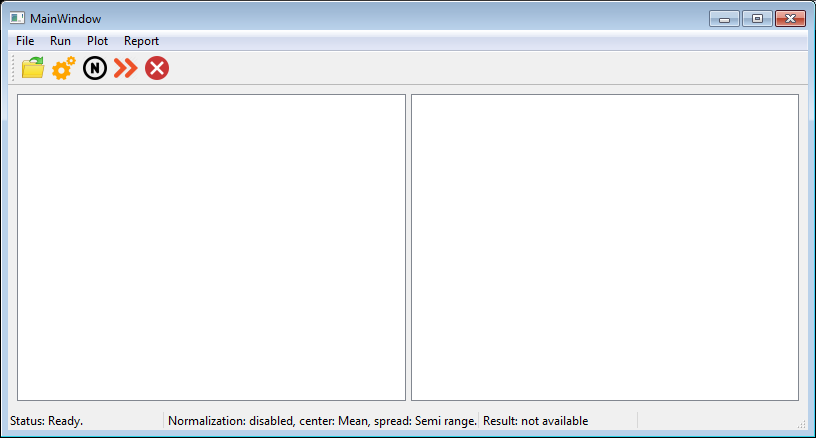
\includegraphics[width=0.95\linewidth]{img/diploma/instruction/empty-window}
		\end{figure}
		
	\end{columns}
	\end{frame}
	
	\begin{frame}{Пользовательское описание программы: загрузка данных}
	\begin{columns}
	\column{0.2\linewidth}
		\begin{figure}[T] % \ContinuedFloat
			\centering
			\includestandalone[width=0.9\linewidth]{img/tikz/stages-vertical-load}
		\end{figure}
	\column{0.8\linewidth}
	\begin{figure}[T] % \ContinuedFloat
		\centering
		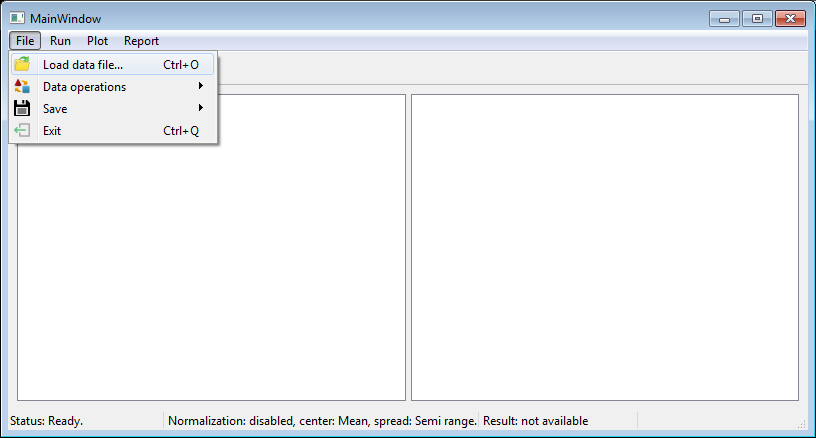
\includegraphics[width=0.95\linewidth]{img/diploma/instruction/open-file-menu}
	\end{figure}

	\end{columns}
	\end{frame}


	\begin{frame}{Пользовательское описание программы: загрузка данных}
	\begin{columns}
		\column{0.2\linewidth}
		\begin{figure}[T] % \ContinuedFloat
			\centering
			\includestandalone[width=0.9\linewidth]{img/tikz/stages-vertical-load}
		\end{figure}
		\column{0.8\linewidth}
		\begin{figure}[T] % \ContinuedFloat
			\centering
			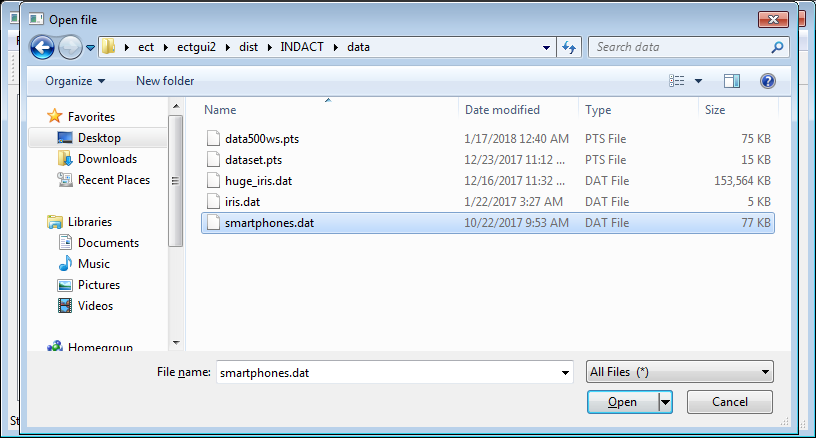
\includegraphics[width=0.95\linewidth]{img/diploma/instruction/open-smartphones-2}
		\end{figure}
	\end{columns}
	\end{frame}
	
	\begin{frame}{Пользовательское описание программы: загрузка данных}
		\begin{columns}
			\column{0.2\linewidth}
			\begin{figure}[T] % \ContinuedFloat
				\centering
				\includestandalone[width=0.9\linewidth]{img/tikz/stages-vertical-load}
			\end{figure}
			\column{0.8\linewidth}
			\begin{figure}[T] % \ContinuedFloat
				\centering
				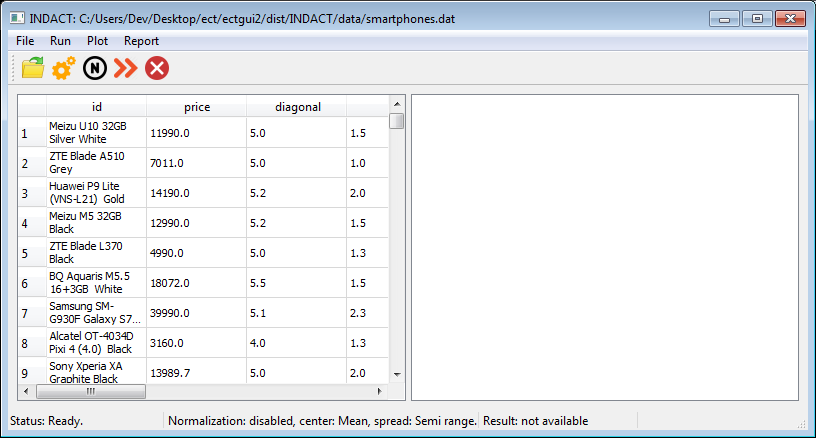
\includegraphics[width=0.95\linewidth]{img/diploma/instruction/load-result-2}
			\end{figure}
		\end{columns}
	\end{frame}


	\begin{frame}{Пользовательское описание программы: нормализация}
		\begin{columns}
			\column{0.2\linewidth}
			\begin{figure}[T] % \ContinuedFloat
				\centering
				\includestandalone[width=0.9\linewidth]{img/tikz/stages-vertical-norm}
			\end{figure}
			\column{0.8\linewidth}
			\begin{figure}[T] % \ContinuedFloat
				\begin{tikzpicture}
					\node[anchor=south west,inner sep=0] (image) at (0,0) {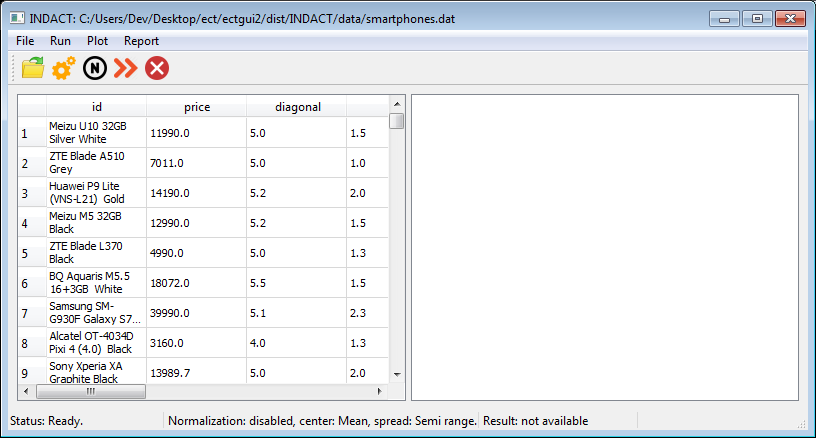
\includegraphics[width=0.95\linewidth]{img/diploma/instruction/load-result-2}};
					\draw[draw=red,fill opacity=0,line width=0.05cm] (0.83cm,4.82cm) circle (0.2cm);
				\end{tikzpicture}
			\end{figure}
		\end{columns}
		\end{frame}

	\begin{frame}{Пользовательское описание программы: нормализация}
	\begin{columns}
		\column{0.2\linewidth}
		\begin{figure}[T] % \ContinuedFloat
			\centering
			\includestandalone[width=0.9\linewidth]{img/tikz/stages-vertical-norm}
		\end{figure}
		\column{0.8\linewidth}
		\begin{figure}[T] % \ContinuedFloat
			\begin{tikzpicture}
			\node[anchor=south west,inner sep=0] (image) at (0,0) {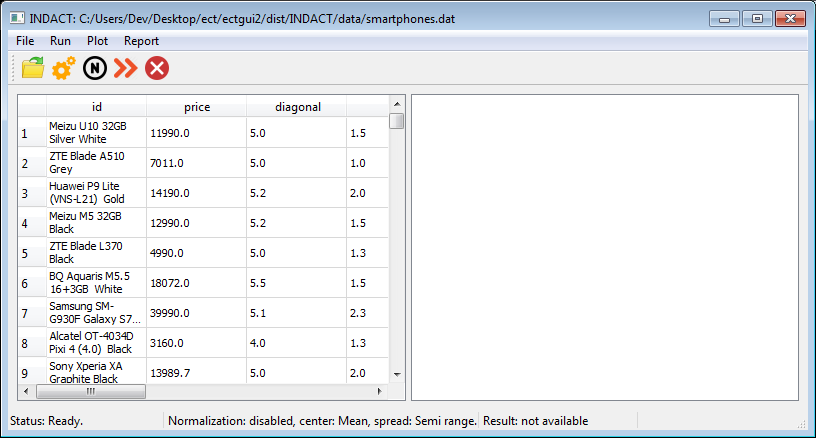
\includegraphics[width=0.95\linewidth]{img/diploma/instruction/load-result-2}};
			\node[anchor=south west,inner sep=0] (image) at (3,2) {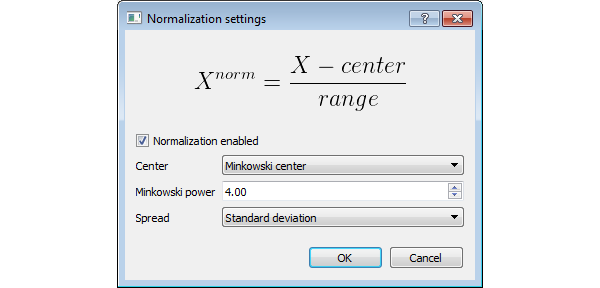
\includegraphics[width=0.60\linewidth]{img/diploma/instruction/mink-norm-params}};
			\end{tikzpicture}
		\end{figure}
	\end{columns}
	\end{frame}

	\begin{frame}{Пользовательское описание программы: нормализация}
	\begin{columns}
		\column{0.2\linewidth}
		\begin{figure}[T] % \ContinuedFloat
			\centering
			\includestandalone[width=0.9\linewidth]{img/tikz/stages-vertical-norm}
		\end{figure}
		\column{0.8\linewidth}
		\begin{figure}[T] % \ContinuedFloat
			\centering
			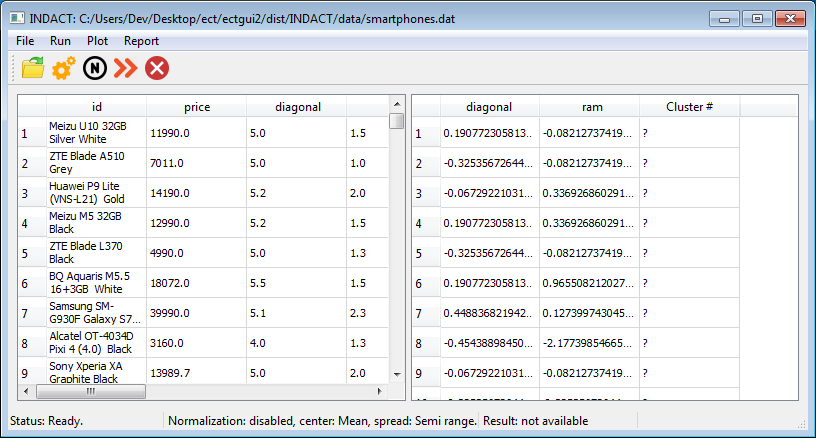
\includegraphics[width=0.95\linewidth]{img/diploma/instruction/norm-result-prez}
		\end{figure}
	\end{columns}
	\end{frame}	


	\begin{frame}{Пользовательское описание программы: кластеризация}
	\begin{columns}
		\column{0.2\linewidth}
		\begin{figure}[T] % \ContinuedFloat
			\centering
			\includestandalone[width=0.9\linewidth]{img/tikz/stages-vertical-clust}
		\end{figure}
		\column{0.8\linewidth}
		\begin{figure}[T] % \ContinuedFloat
			\centering
			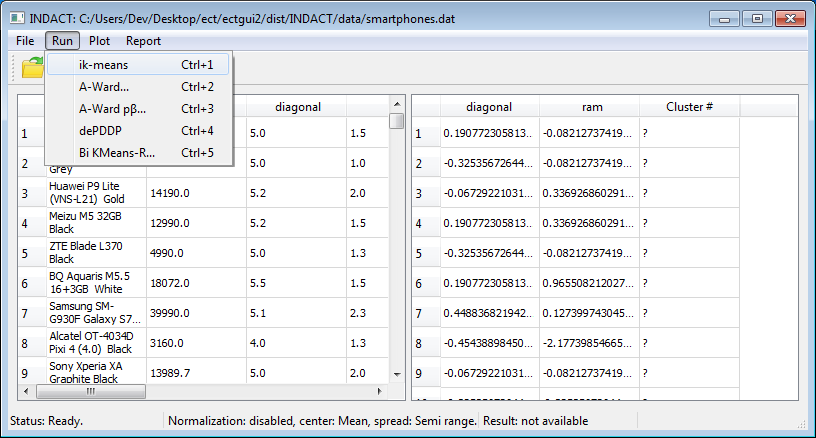
\includegraphics[width=0.95\linewidth]{img/diploma/instruction/run-clustering-prez}
		\end{figure}
	\end{columns}
	\end{frame}	

	\begin{frame}{Пользовательское описание программы: кластеризация}
		\begin{columns}
			\column{0.2\linewidth}
			\begin{figure}[T] % \ContinuedFloat
				\centering
				\includestandalone[width=0.9\linewidth]{img/tikz/stages-vertical-clust}
			\end{figure}
			\column{0.8\linewidth}
			\begin{figure}[T] % \ContinuedFloat
				\begin{tikzpicture}
				\node[anchor=south west,inner sep=0] (image) at (0,0) {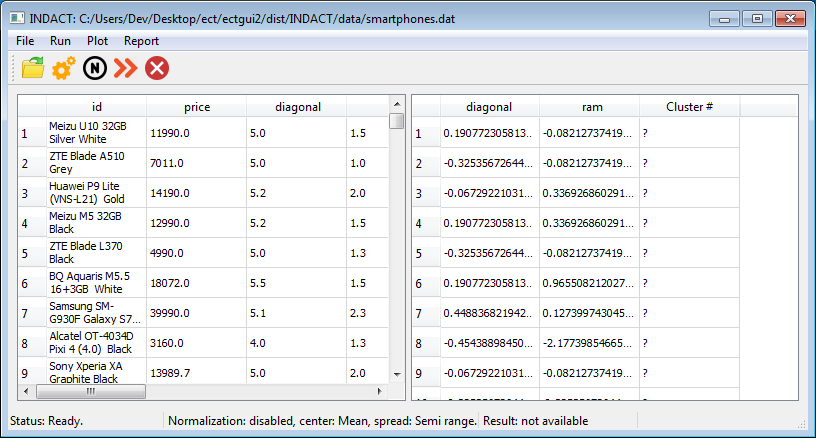
\includegraphics[width=0.95\linewidth]{img/diploma/instruction/norm-result-prez}};
				\node[anchor=south west,inner sep=0] (image) at (2,1) {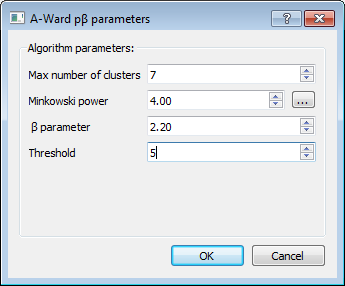
\includegraphics[width=0.40\linewidth]{img/diploma/instruction/tutorial-awardpb-settings}};
				\end{tikzpicture}
			\end{figure}
		\end{columns}
	\end{frame}	


	\begin{frame}{Пользовательское описание программы: кластеризация}
		\begin{columns}
			\column{0.2\linewidth}
			\begin{figure}[T] % \ContinuedFloat
				\centering
				\includestandalone[width=0.9\linewidth]{img/tikz/stages-vertical-clust}
			\end{figure}
			\column{0.8\linewidth}
			\begin{figure}[T] % \ContinuedFloat
				\centering
				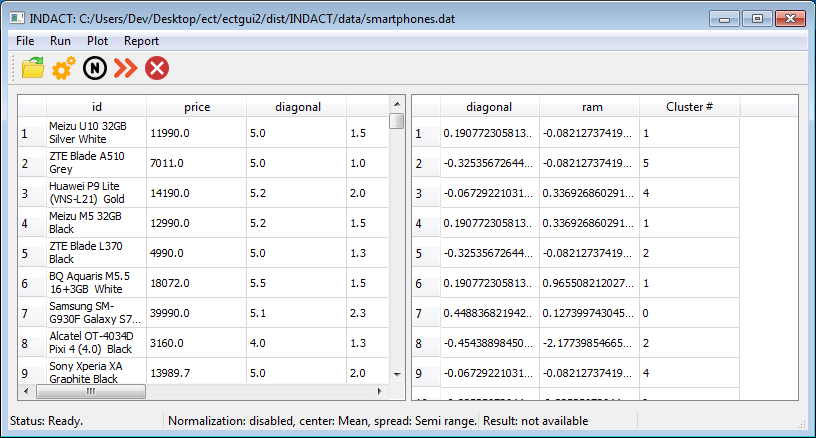
\includegraphics[width=0.95\linewidth]{img/diploma/instruction/clustering-compl1-prez}
			\end{figure}
		\end{columns}
	\end{frame}	
	
	
	\begin{frame}{Пользовательское описание программы: кластеризация}
	\begin{columns}
		\column{0.2\linewidth}
		\begin{figure}[T] % \ContinuedFloat
			\centering
			\includestandalone[width=0.9\linewidth]{img/tikz/stages-vertical-clust}
		\end{figure}
		\column{0.8\linewidth}
		\begin{figure}[T] % \ContinuedFloat
			\centering
			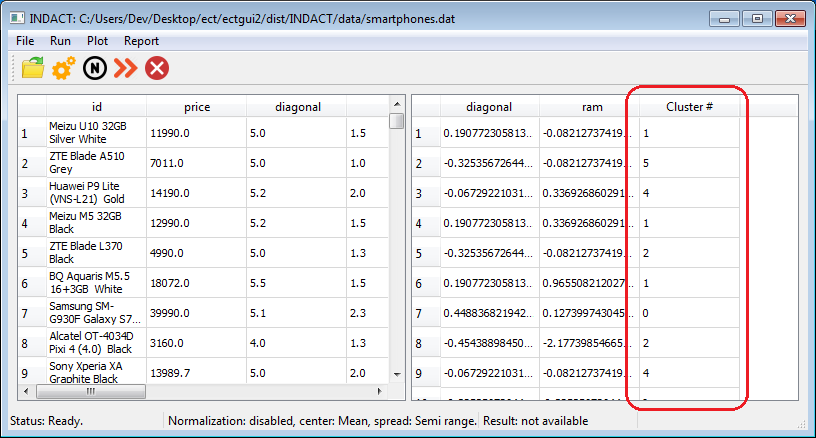
\includegraphics[width=0.95\linewidth]{img/diploma/instruction/clustering-compl2-prez}
		\end{figure}
	\end{columns}
	\end{frame}	

	\begin{frame}{Пользовательское описание программы: анализ}
	\begin{columns}
		\column{0.2\linewidth}
		\begin{figure}[T] % \ContinuedFloat
			\centering
			\includestandalone[width=0.9\linewidth]{img/tikz/stages-vertical-an}
		\end{figure}
		\column{0.8\linewidth}
		\begin{figure}[T] % \ContinuedFloat
			\centering
			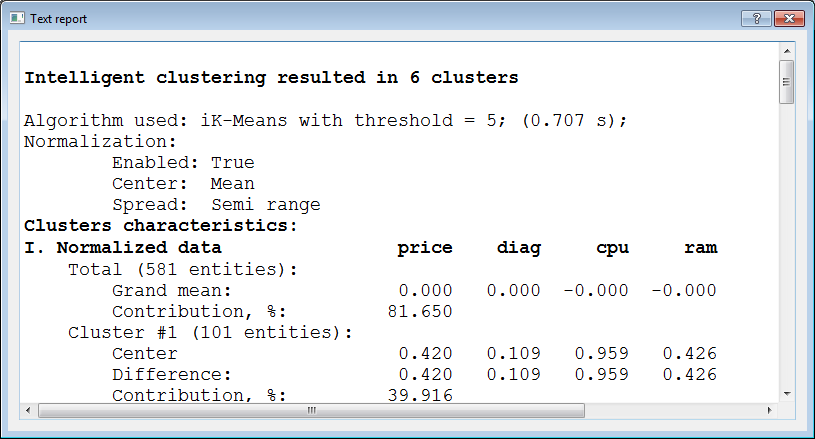
\includegraphics[width=0.95\linewidth]{img/diploma/instruction/text-report}
		\end{figure}
	\end{columns}
	\end{frame}	

	\begin{frame}{Пользовательское описание программы: анализ}
	\begin{columns}
		\column{0.2\linewidth}
		\begin{figure}[T] % \ContinuedFloat
			\centering
			\includestandalone[width=0.9\linewidth]{img/tikz/stages-vertical-an}
		\end{figure}
		\column{0.8\linewidth}
		\begin{figure}[T] % \ContinuedFloat
			\begin{tikzpicture}
			\node[anchor=south west,inner sep=0] (image) at (0,0) {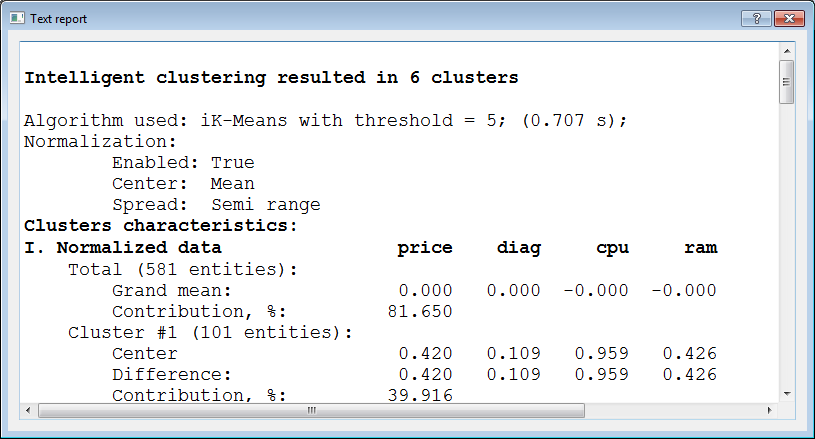
\includegraphics[width=0.95\linewidth]{img/diploma/instruction/text-report}};
			\node[anchor=south west,inner sep=0] (image) at (0.5,-0.25) {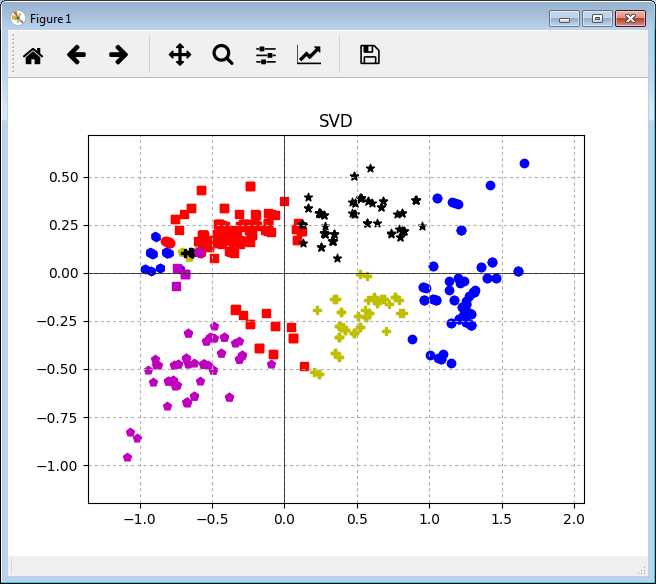
\includegraphics[width=0.55\linewidth]{img/diploma/instruction/tutorial-svd-result}};
			\end{tikzpicture}
		\end{figure}
	\end{columns}
	\end{frame}	

	\begin{frame}{Пользовательское описание программы: анализ}
	\begin{columns}
		\column{0.2\linewidth}
		\begin{figure}[T] % \ContinuedFloat
			\centering
			\includestandalone[width=0.9\linewidth]{img/tikz/stages-vertical-an}
		\end{figure}
		\column{0.8\linewidth}
		\begin{figure}[T] % \ContinuedFloat
			\begin{tikzpicture}
			\node[anchor=south west,inner sep=0] (image) at (0,0) {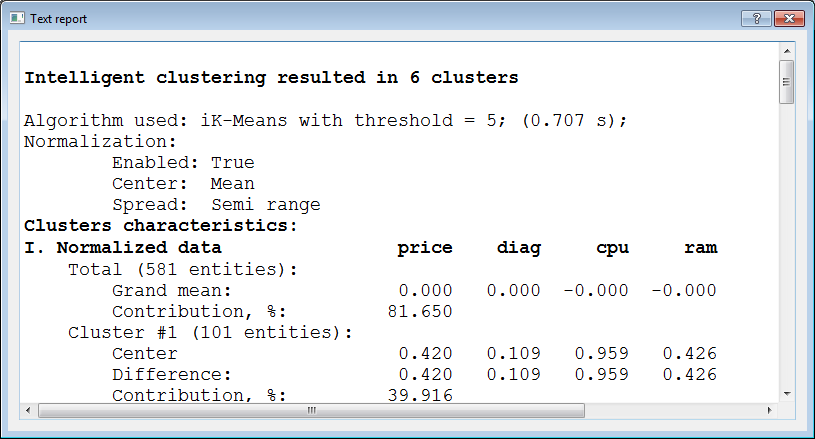
\includegraphics[width=0.95\linewidth]{img/diploma/instruction/text-report}};
			\node[anchor=south west,inner sep=0] (image) at (0.5,-0.25) {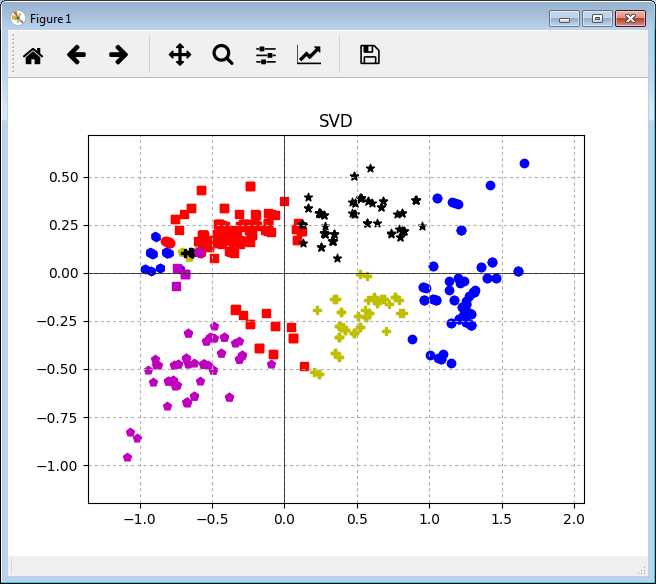
\includegraphics[width=0.55\linewidth]{img/diploma/instruction/tutorial-svd-result}};
			\node[anchor=south west,inner sep=0] (image) at (1,-0.5) {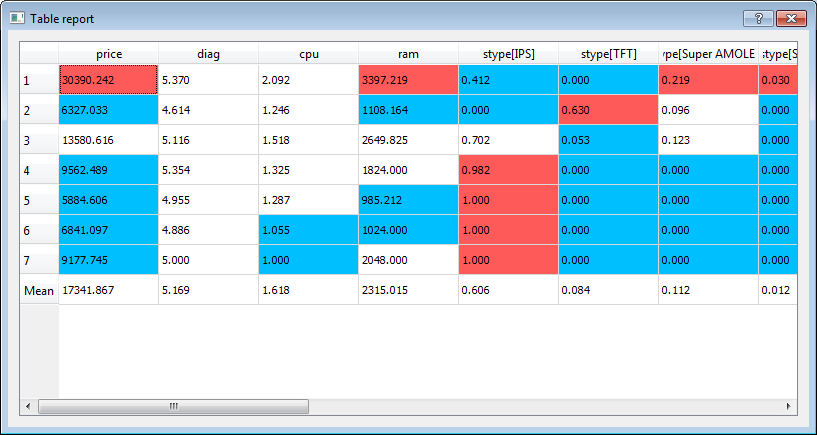
\includegraphics[width=0.85\linewidth]{img/diploma/instruction/tutorial-view-table-report}};
			\end{tikzpicture}
		\end{figure}
	\end{columns}
	\end{frame}	


	\begin{frame}{Пользовательское описание программы: анализ}
	\begin{columns}
		\column{0.2\linewidth}
		\begin{figure}[T] % \ContinuedFloat
			\centering
			\includestandalone[width=0.9\linewidth]{img/tikz/stages-vertical-an}
		\end{figure}
		\column{0.8\linewidth}
		\begin{figure}[T] % \ContinuedFloat
			\begin{tikzpicture}
			\node[anchor=south west,inner sep=0] (image) at (0,0) {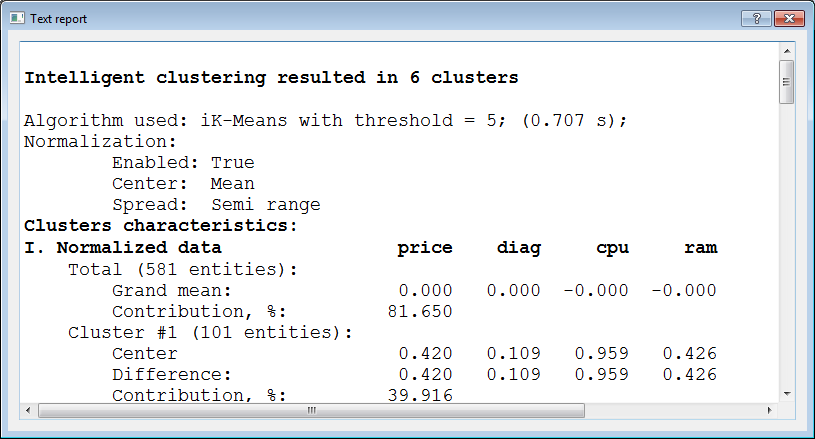
\includegraphics[width=0.95\linewidth]{img/diploma/instruction/text-report}};
			\node[anchor=south west,inner sep=0] (image) at (0.5,-0.25) {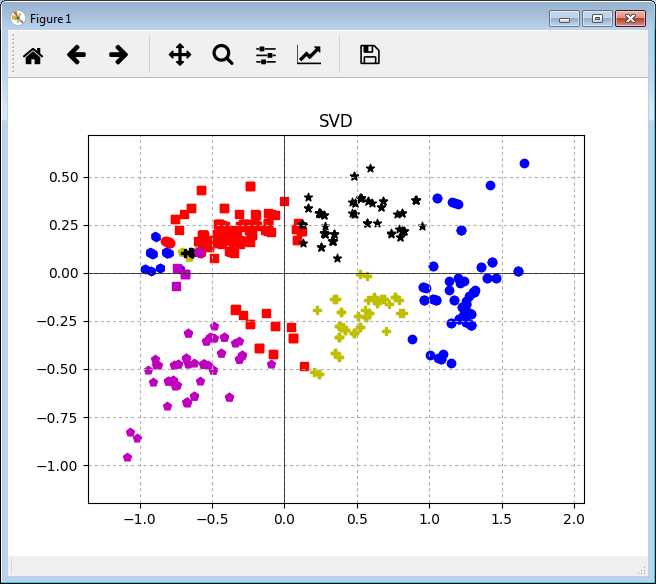
\includegraphics[width=0.55\linewidth]{img/diploma/instruction/tutorial-svd-result}};
			\node[anchor=south west,inner sep=0] (image) at (1,-0.5) {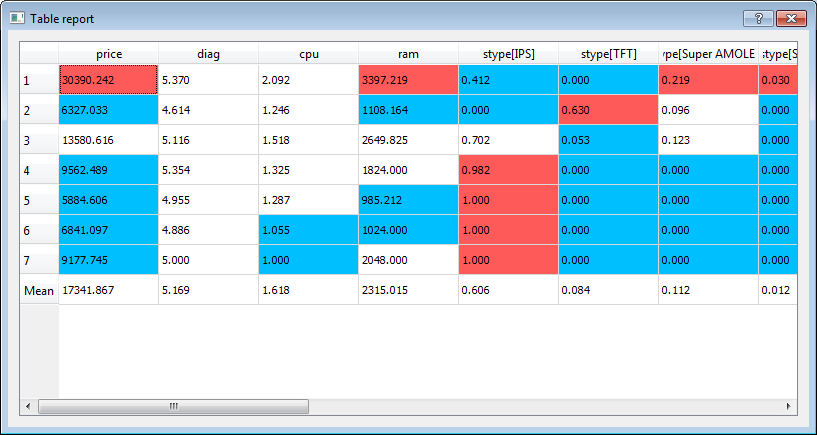
\includegraphics[width=0.85\linewidth]{img/diploma/instruction/tutorial-view-table-report}};
			\node[anchor=south west,inner sep=0] (image) at (1.5,-0.75) {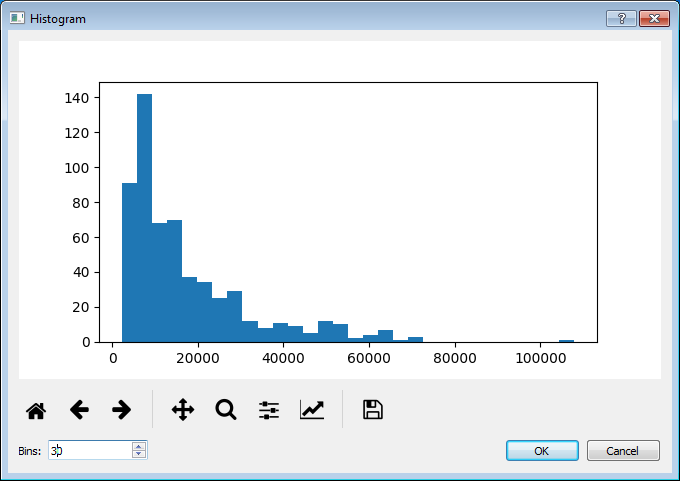
\includegraphics[width=0.85\linewidth]{img/diploma/instruction/hist-set-bins}};
			\end{tikzpicture}
		\end{figure}
	\end{columns}
	\end{frame}	

%	\section{Внутренняя организация}

	\begin{frame}{Внутренняя организация: основные сведения}
	\begin{itemize}
		\item \textbf{Язык:} Python 3\\
		\item \textbf{GUI:} PyQt\\
		\item \textbf{Библиотеки:} Pandas, NumPy, SciPy, scikit-learn, Matplotlib
		\item \textbf{Тестирование:} pytest
		\item \textbf{Дистрибуция:} pyinstaller
	\end{itemize}
	\end{frame}

	\begin{frame}{Внутренняя организация: структура пакетов}
		\begin{figure}[T] % \ContinuedFloat
		\centering
		\includestandalone[height=0.9\textheight]{img/tikz/packages}
		\end{figure}
	\end{frame}

	\begin{frame}{Внутренняя организация: диаграмма классов}
	\begin{figure}[T] % \ContinuedFloat
		\centering
		\includestandalone[height=0.9\textheight]{img/tikz/ap-init-classes}
	\end{figure}
	\end{frame}

%	\section{Демонстрационный пример}

	\begin{frame}{Демонстрационный пример: описание исходных данных}
	\begin{itemize}
		\item \textbf{Размерность:} 386 $ \times $ 4\\
		\item \textbf{Предметная область:} модели смартфонов \\
		\item \textbf{Источник:} www.ozon.ru/context/partner\_xml \\
		\item \textbf{Признаки:}\\
		\begin{table}[h!]
			\begin{tabular}{|C{0.04\linewidth}| C{0.15\linewidth} | L{0.45\linewidth} | C{0.24\linewidth}| }
				\hline \# & Название & Описание  & Единица измерения\\ 
				\hline 1 & price & Цена данной модели смартфона в IV квартале 2017 года & руб. \\ 
				\hline 2 & diag & Размер диагонали экрана & дюйм \\
				\hline 3 & cpu & Частота центрального процессора (ЦП) & ГГц \\			
				\hline 4 & ram & Объем оперативной памяти & Мб \\						
				\hline
			\end{tabular}
		\end{table}

	\end{itemize}
	\end{frame}
	
	

	\begin{frame}{Демонстрационный пример: фрагмент данных}
		\vspace{0.4cm}
		\lstinputlisting[basicstyle=\ttfamily\scriptsize, numbers=none,firstline=0,lastline=17,language={}]{code/smartphones.dat}
	\end{frame}

	\begin{frame}{Демонстрационный пример: SVD представления разбиений}
		
		\begin{figure}[T] % \ContinuedFloat
			\begin{tikzpicture}
			\node[anchor=south west,inner sep=0] (image) at (-1.5,3.8) {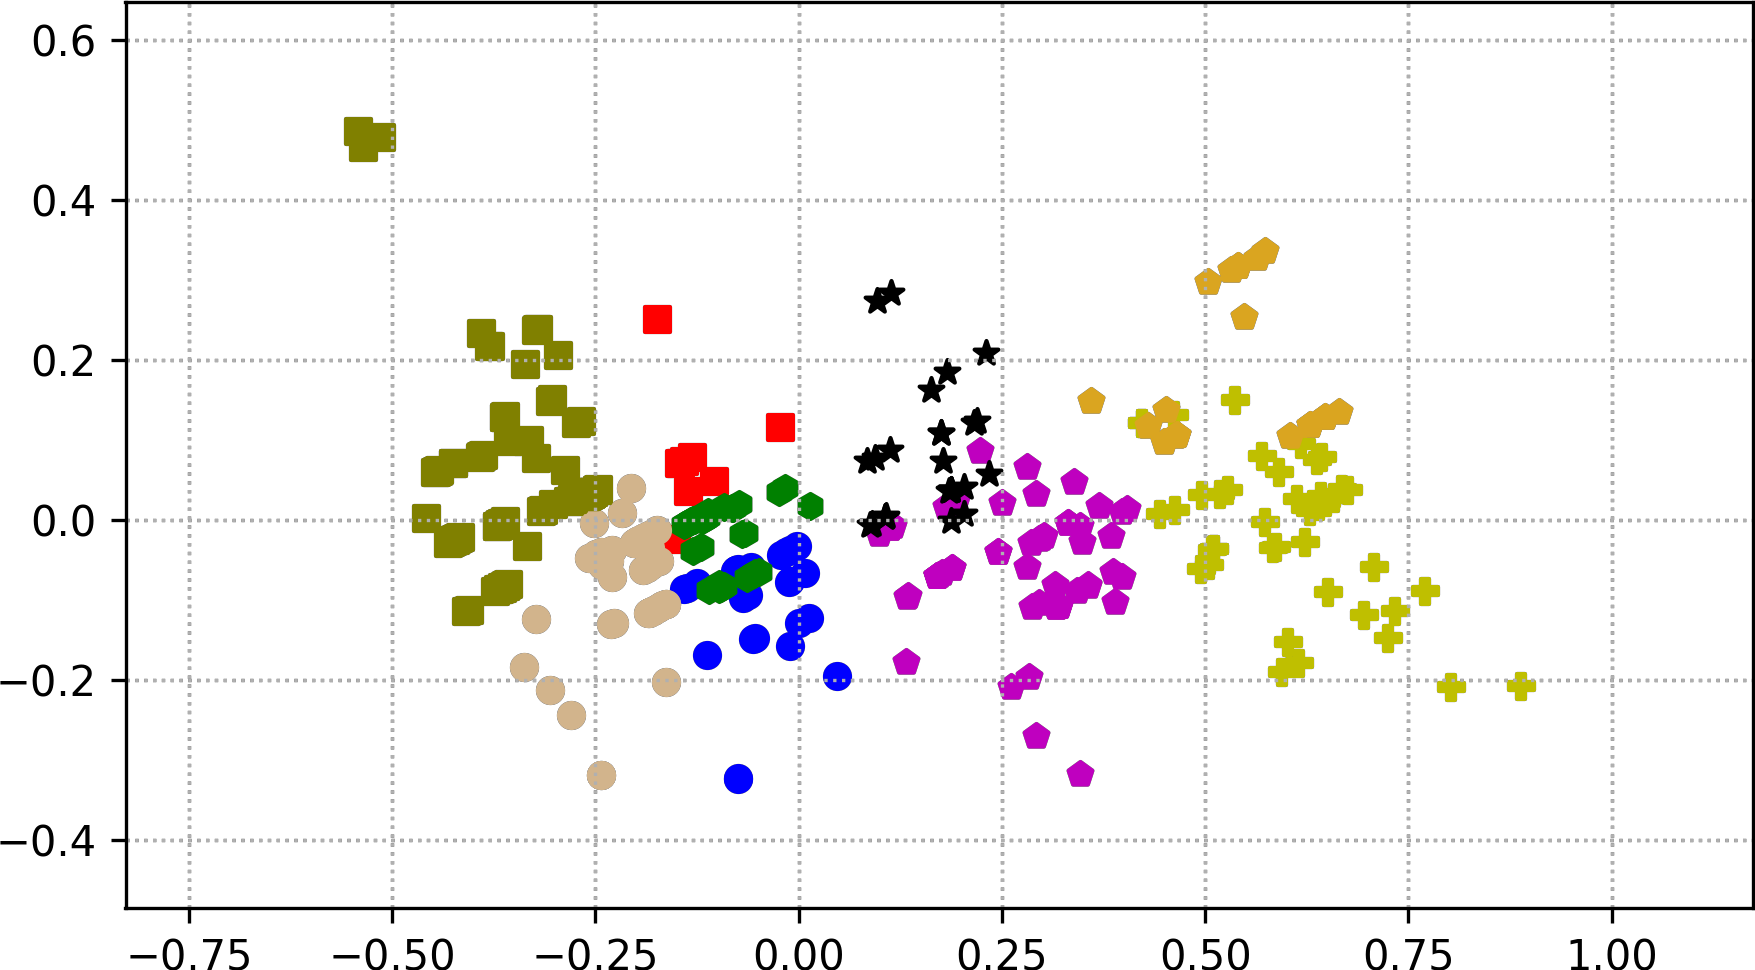
\includegraphics[width=0.45\linewidth]{img/svd/ikmeans-svd}};
			\node[anchor=south west,inner sep=0] (image) at (5.5,3.8) {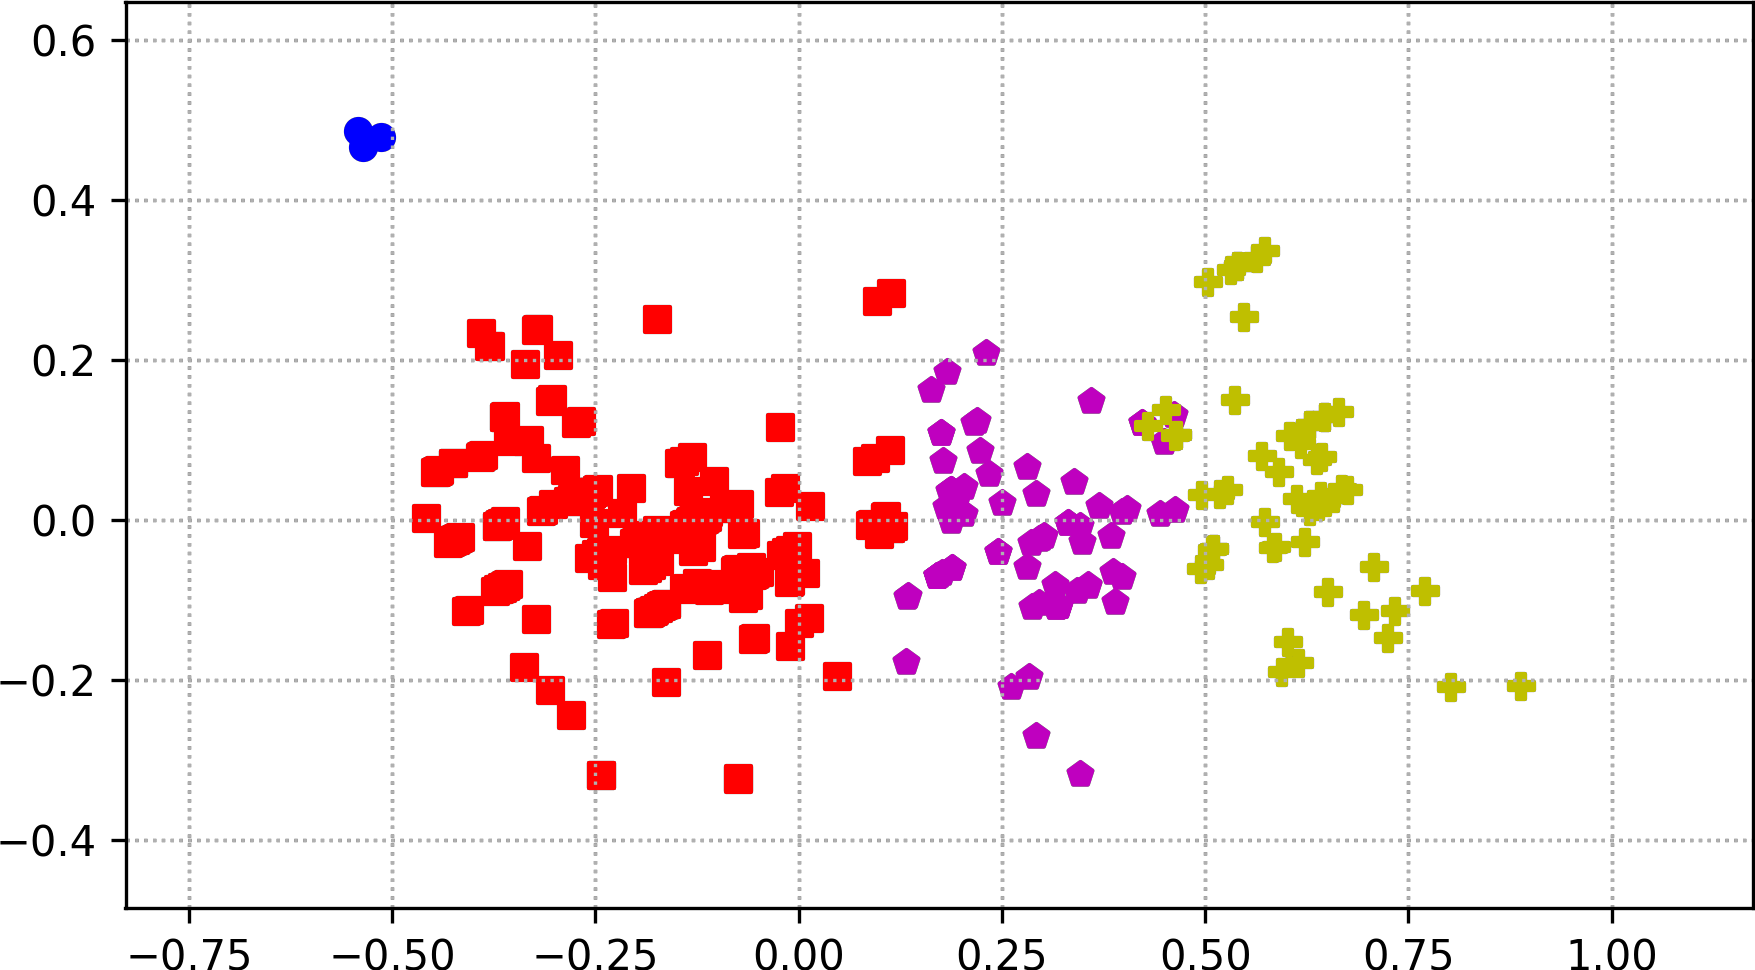
\includegraphics[width=0.45\linewidth]{img/svd/depddp-svd}};
			\node[anchor=south west,inner sep=0] (image) at (-1.5,0) {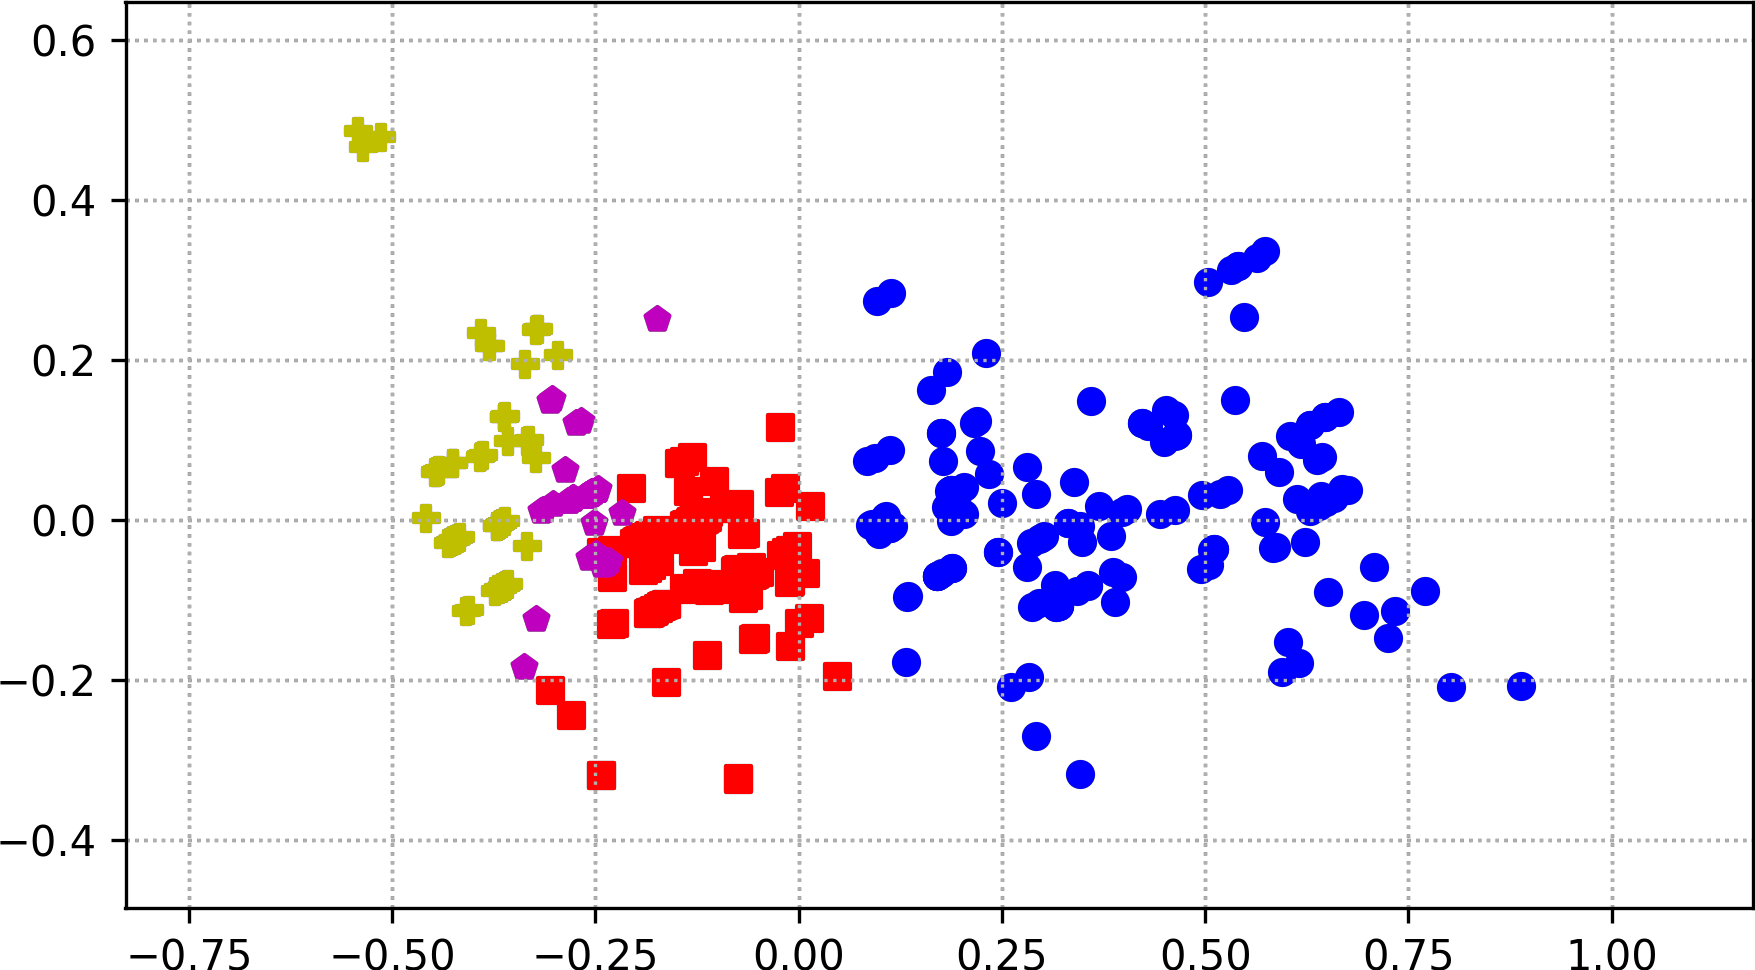
\includegraphics[width=0.45\linewidth]{img/svd/bikmr-svd}};
			\node[anchor=south west,inner sep=0] (image) at (5.5,0) {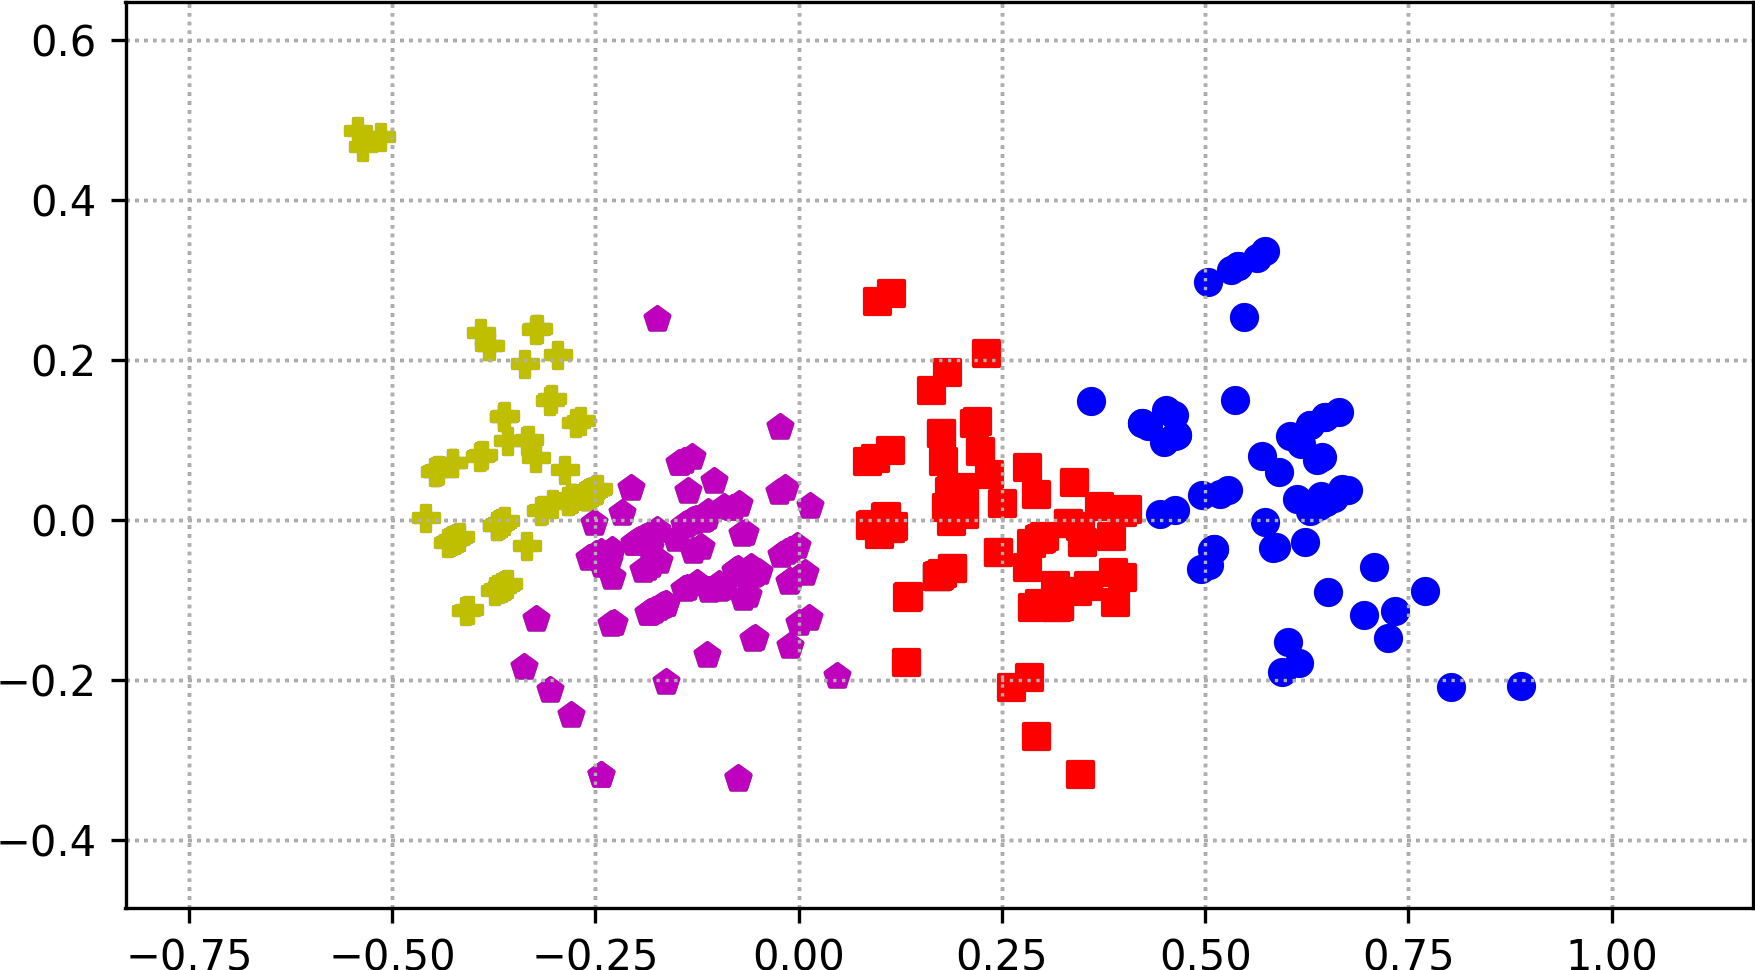
\includegraphics[width=0.45\linewidth]{img/svd/award-svd}};
			\node [draw=none,anchor=west, xshift=0cm, rotate=90,anchor=north,outer sep=-4pt, font=\small, ] at (-1.9,5.5) {\ikmeans (9)};
			\node [draw=none,anchor=west, xshift=0cm, rotate=90,anchor=north,outer sep=-4pt, font=\small, ] at (5.1,5.5) {\dePDDP (4)};
			
			\node [draw=none,anchor=west, xshift=0cm, rotate=90,anchor=north,outer sep=-4pt, font=\small, ] at (-1.9,2) {\BiKMR (4)};
			\node [draw=none,anchor=west, xshift=0cm, rotate=90,anchor=north,outer sep=-4pt, font=\small, ] at (5.1,2) {\AWard (4*)};
			\end{tikzpicture}
		\end{figure}
		
%		\begin{figure}[h!] % \ContinuedFloat
%			\centering
%			\subfigure[\ikmeans] {\label{fig:svd-sample1}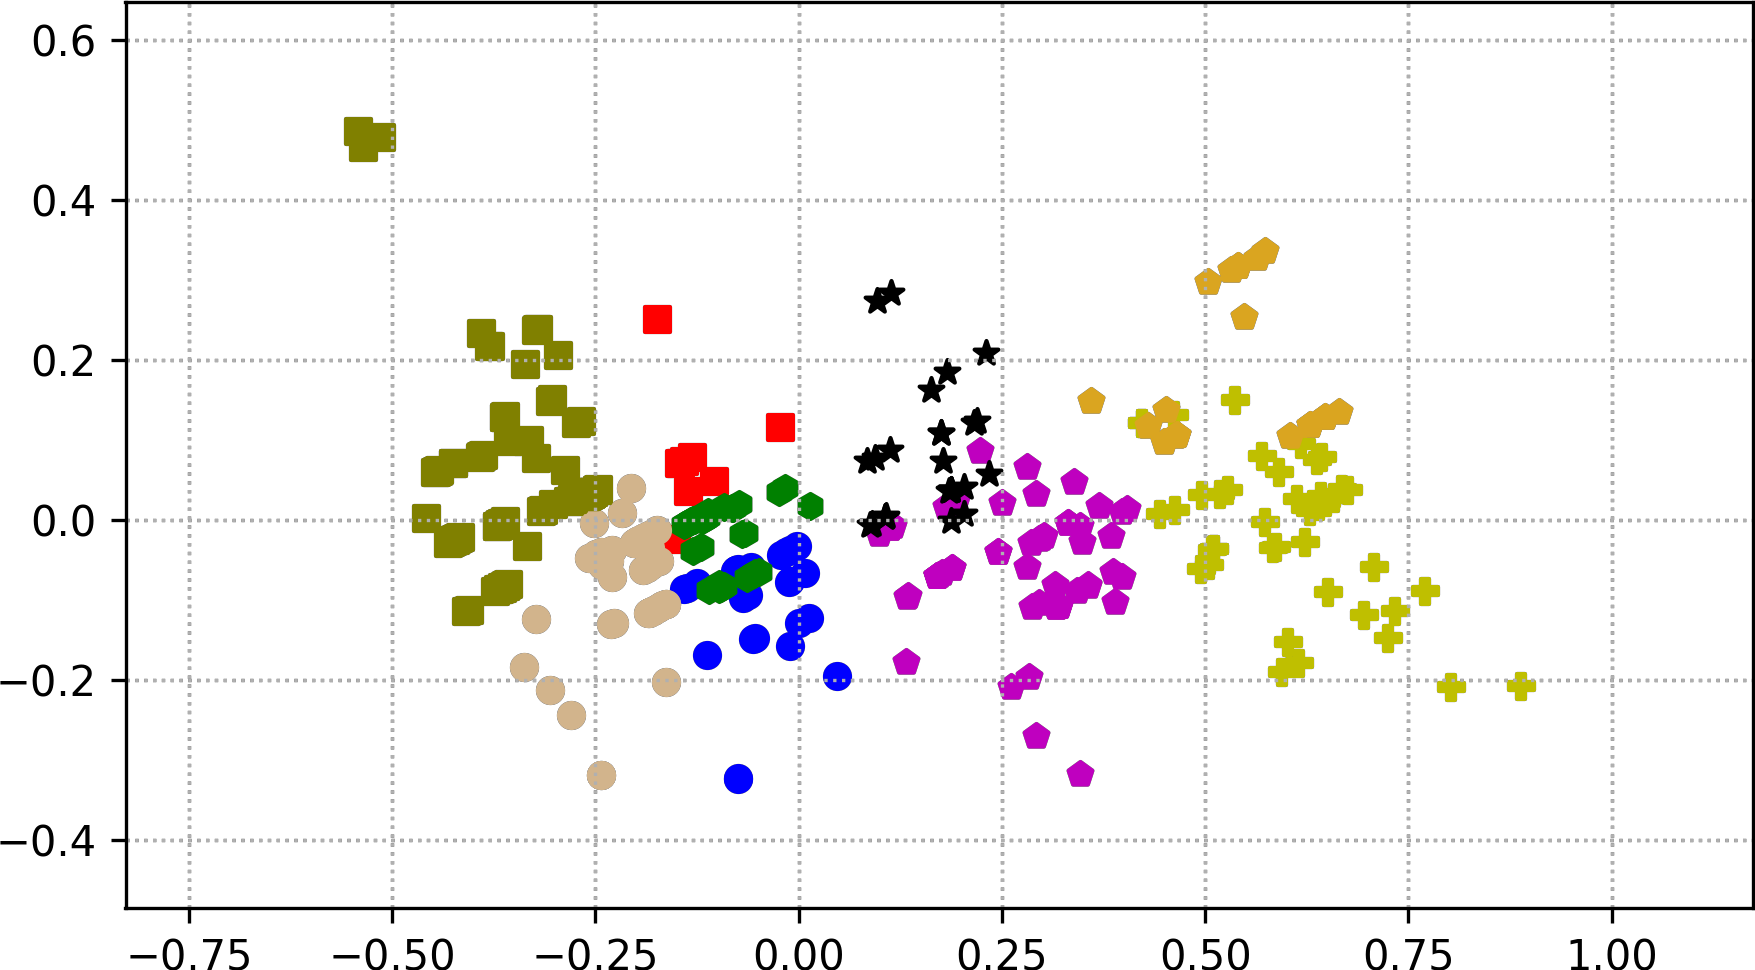
\includegraphics[height=0.17\linewidth]{img/svd/ikmeans-svd}}
%			\subfigure[\dePDDP]  {\label{fig:svd-sample2}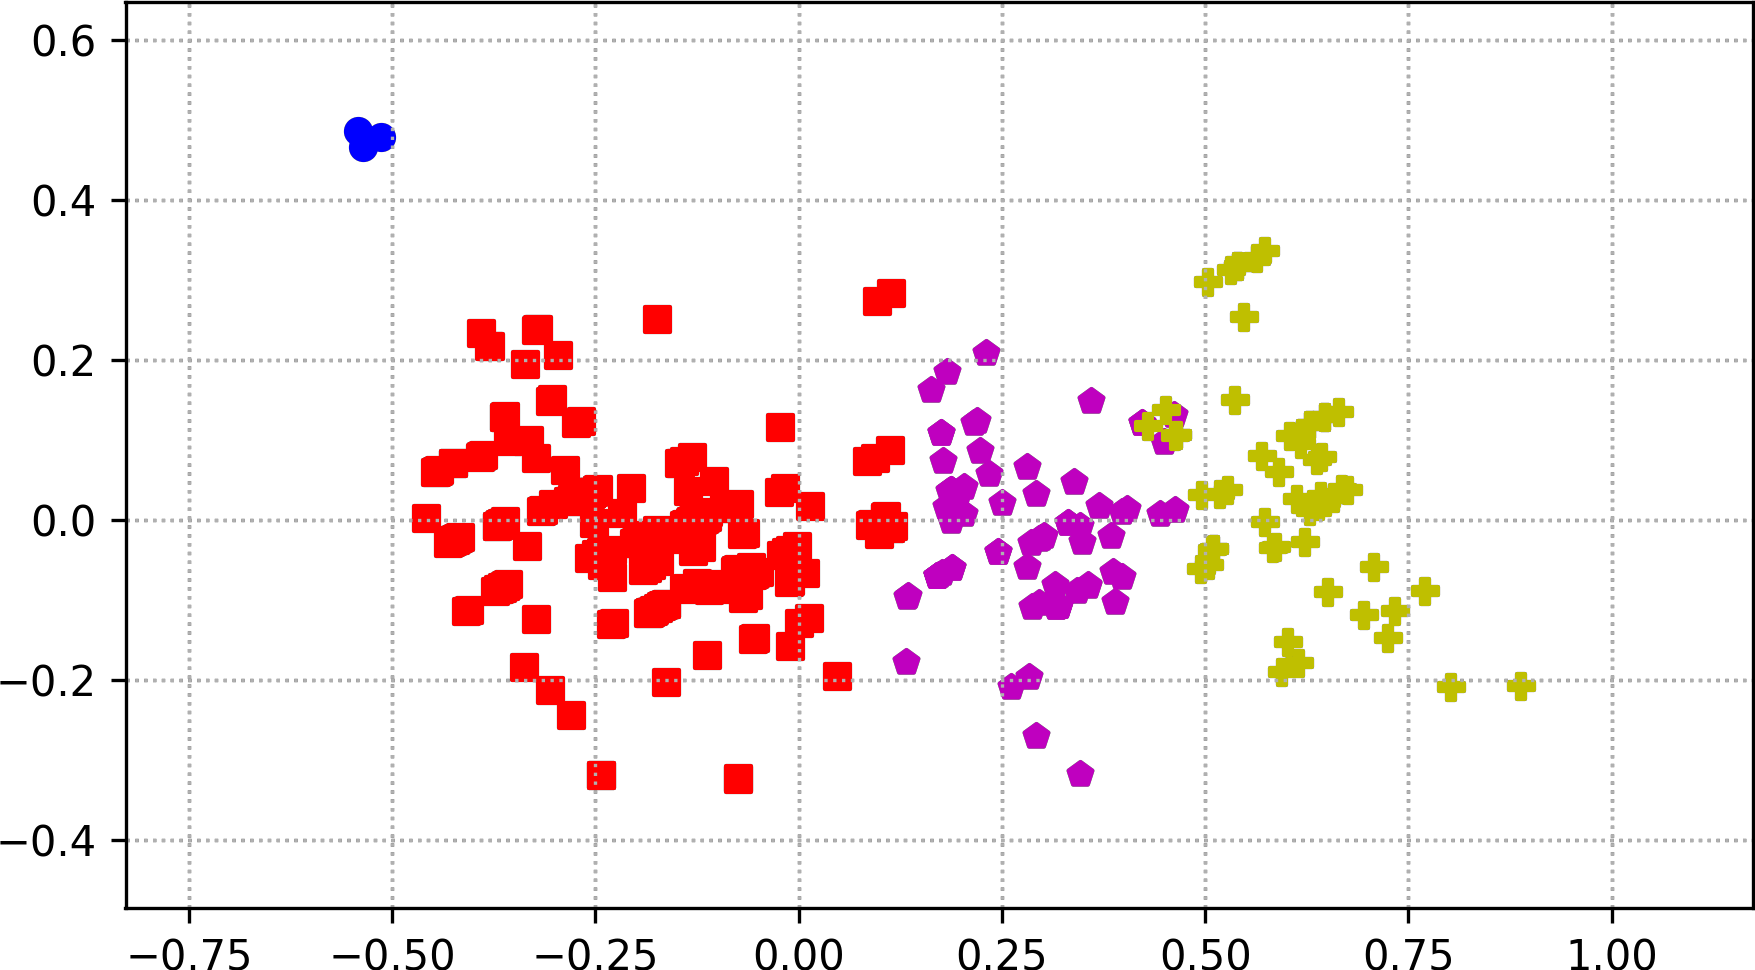
\includegraphics[height=0.17\linewidth]{img/svd/depddp-svd}}
%			\subfigure[\BiKMR]   {\label{fig:svd-sample3}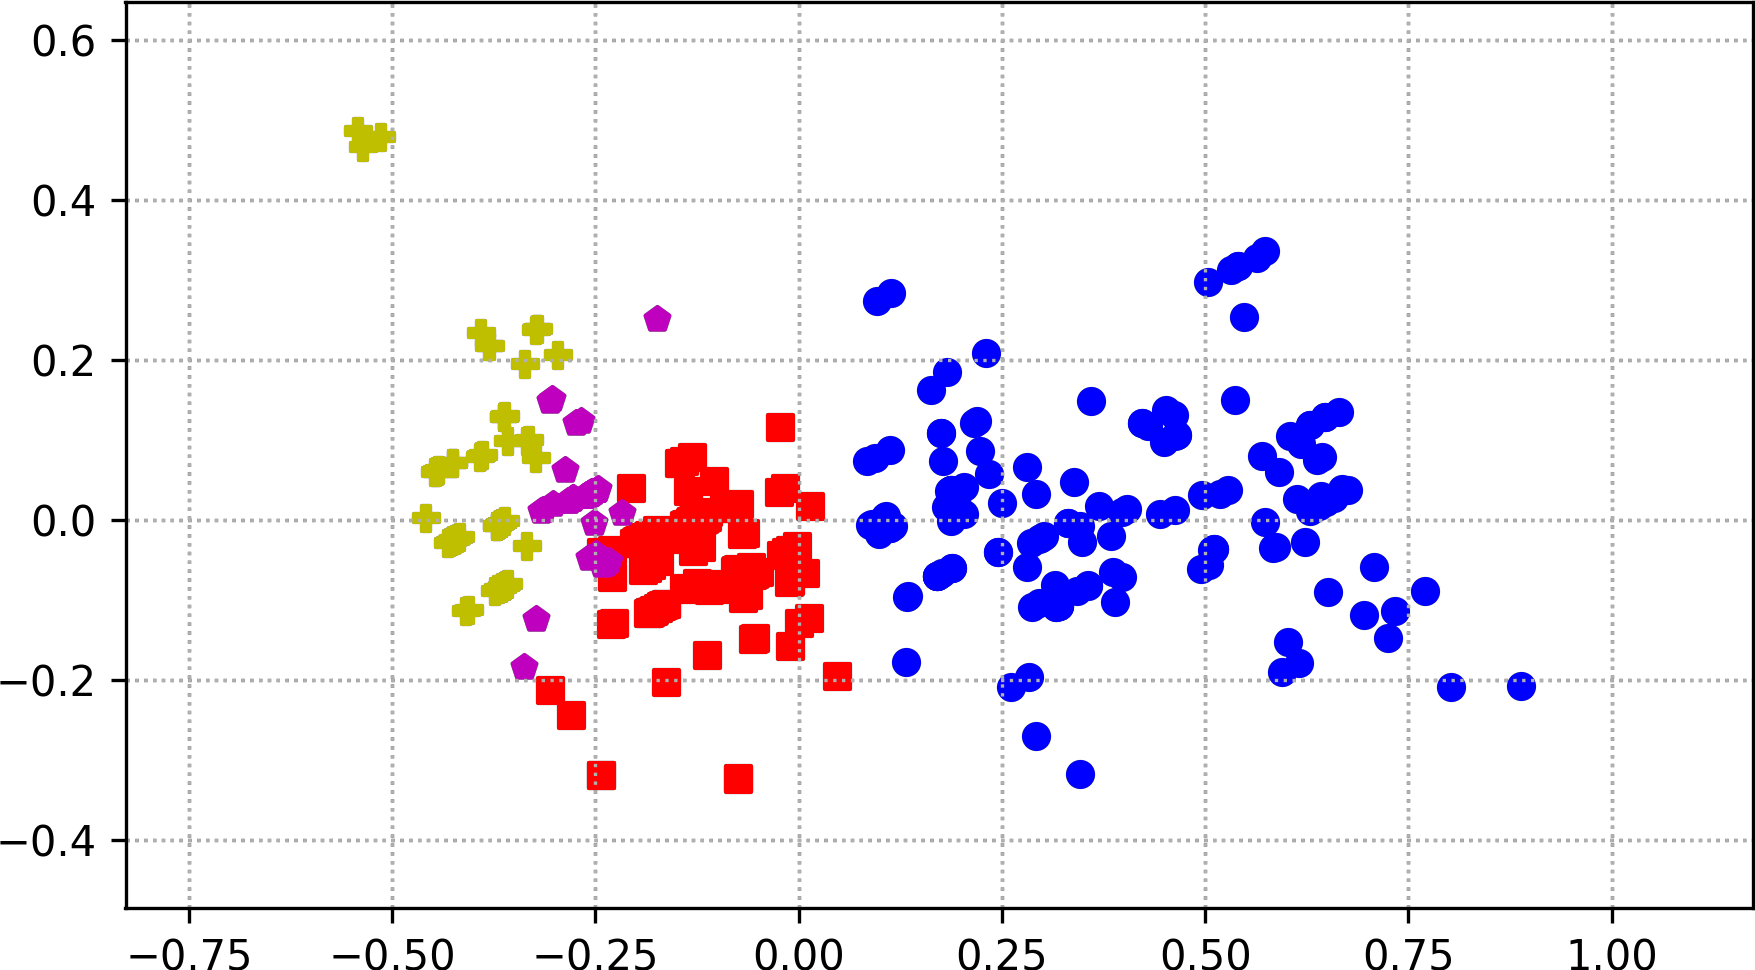
\includegraphics[height=0.17\linewidth]{img/svd/bikmr-svd}}		
%			\subfigure[\AWard]   {\label{fig:svd-sample4}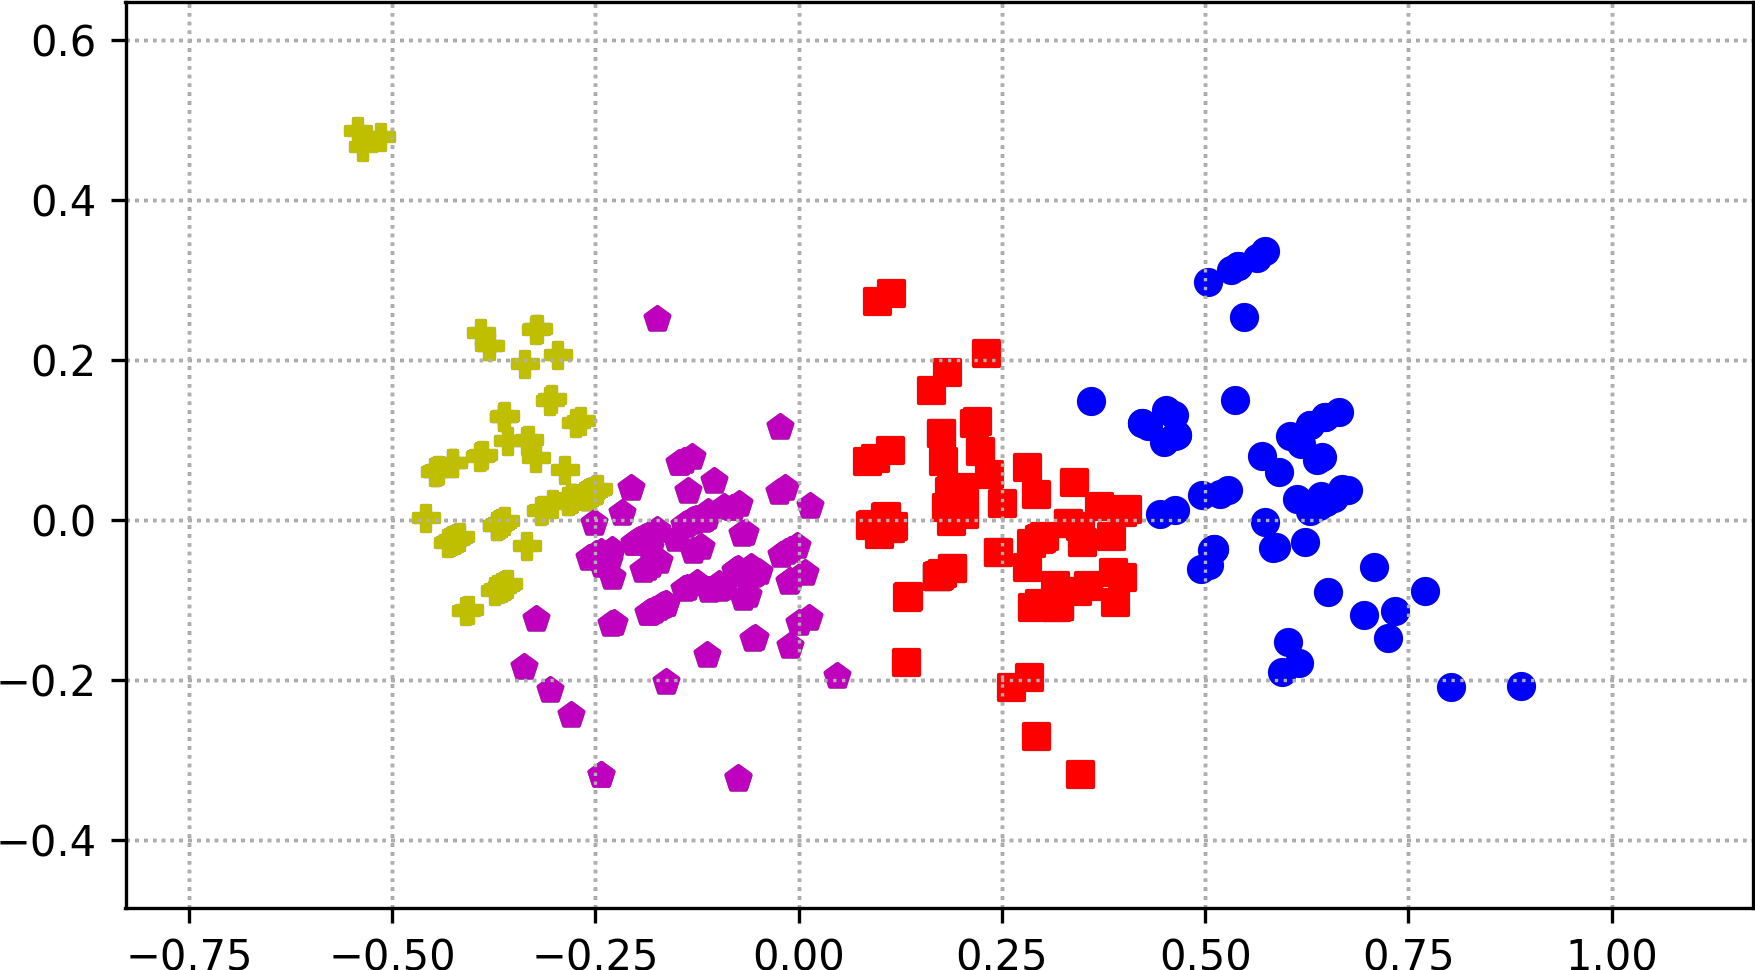
\includegraphics[height=0.17\linewidth]{img/svd/award-svd}}
%		\end{figure}	
	\end{frame}


	\begin{frame}{Демонстрационный пример: попарный индекс ARI}
	\begin{table}[]
		\centering
%		\caption{Попарный индекс ARI полученных разбиений}
%		\label{tab:alg-ari}	
		\begin{tabular}{|c|c|c|c|c|c|}
			\hline
			Число кластеров & Алгоритм & \ikmeans & \dePDDP & \BiKMR & \AWard \\ 
			\hline
			9 & \ikmeans  & 1 & 0.28 & 0.36  & 0.67  \\ 
			\hline
			4  & \dePDDP  & - & 1 & 0.25 & 0.46 \\ 
			\hline
			4   & \BiKMR  & - & - & 1 & 0.63 \\ 
			\hline
			4*   & \AWard & - & - & - & 1\\
			\hline
		\end{tabular} 
	\end{table}
	\end{frame}


	\begin{frame}{Демонстрационный пример: интерпретация результатов -- \AWard}
	\begin{figure}[h] % \ContinuedFloat
		\centering
		\includestandalone[width=0.98\textwidth]{img/tikz/interpretation-award}
%		\subfigure[\dePDDP]  {\label{fig:interp2}\includestandalone[width=0.98\textwidth]{img/tikz/interpretation-depddp2}}
%		\subfigure[\AWard]   {\label{fig:interp4}\includestandalone[width=0.98\textwidth]{img/tikz/interpretation-award}}
%		\caption{Относительное отклонение от среднего признаков в кластерах}
%		\label{fig:interp}
	\end{figure}		
	\end{frame}

	\begin{frame}{Демонстрационный пример: интерпретация результатов -- \dePDDP}
	\begin{figure}[h] % \ContinuedFloat
		\centering
		\includestandalone[width=0.98\textwidth]{img/tikz/interpretation-depddp2}
		%		\subfigure[\dePDDP]  {\label{fig:interp2}\includestandalone[width=0.98\textwidth]{img/tikz/interpretation-depddp2}}
		%		\subfigure[\AWard]   {\label{fig:interp4}\includestandalone[width=0.98\textwidth]{img/tikz/interpretation-award}}
		%		\caption{Относительное отклонение от среднего признаков в кластерах}
		%		\label{fig:interp}
	\end{figure}		
	\end{frame}

		
	\plain{	
		\textsc{Выводы}
		\begin{enumerate}
			\item \textbullet~Реализована система, включающая 5 современных алгоритмов 
			\item \textbullet~При разработке учтены тенденции в области проектирования ПО
			\item \textbullet~INDACT позволит облегчить применение разработанных алгоритмов 
			\item 
		\end{enumerate}
		}
	
	\plain{
		\textsc{Спасибо за внимание}!
		}
	

	
\end{document}


